\documentclass[12pt]{article} 
\usepackage{graphicx} 
\usepackage{titlesec}

% Replace `letterpaper' with `a4paper' for UK/EU standard size
\usepackage[a4paper,top=2cm,bottom=2cm,left=3cm,right=3cm,marginparwidth=1.75cm]{geometry}

% Useful packages
\usepackage{amsmath}
\usepackage{graphicx}
\usepackage{tabularx} % Include the tabularx package
\usepackage{hyperref}
\usepackage{caption}
\usepackage{subcaption}
\usepackage{caption}
\usepackage{subcaption}
\usepackage{placeins}

% Center section headings
\titleformat{\section}
  {\normalfont\Large\bfseries}
  {\thesection}
  {1em}
  {}
 

\begin{document}

\begin{titlepage}
\centering
\vspace{0.5cm}
{\Huge\bfseries Pruning and Sparsity\par}

\vspace{0.5cm} % Adds vertical space
{\Large SAiDL 2024 Assignment}

\vspace{1.5cm}
{\Large Sasmit Datta}
\end{titlepage}

%%%%%%%%%%%%%%%%%%%%%%%%%%%%%%%%%%%%%%%%%%%%%%%
\section{Introduction}
In the pursuit of creating more efficient and scalable deep learning models, pruning stands out as an essential technique to reduce model size and computational complexity without significantly compromising accuracy. Along with \textbf{fine-grained} pruning on a CNN trained on the CIFAR-10 dataset, I implement \textbf{kernel} and \textbf{filter} pruning and present a comprehensive analysis on the same.

%%%%%%%%%%%%%%%%%%%%%%%%%%%%%%%%%%%%%%%%%%%%%%%
\section{Pruning Strategies}
All the pruning strategies are implemented using magnitude based approaches - more specifically by calculating the norm of a weight or a series of weights.

\subsection{Fine-grained}
Fine-grained pruning, often referred to as unstructured pruning, involves the selective removal of individual weights across the network based on their magnitudes.

\begin{figure}[h]
\centering
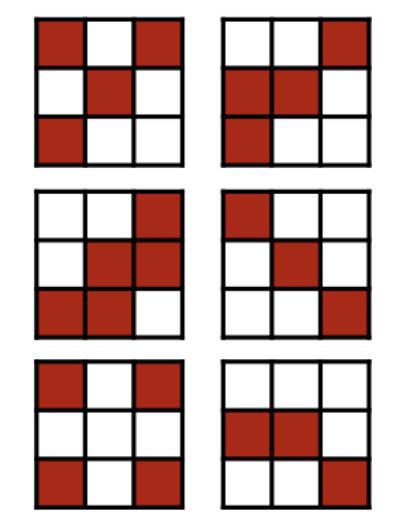
\includegraphics[width=0.2\linewidth]{report_images/fine_pruning.png}
\caption{\label{fig:fine_pruning_diag}Fine-grained Pruning}
\end{figure}

\noindent
Provided sparsity value $s\%$ for a particular layer, $s\%$ of weights with lower absolute values are pruned.
\begin{equation}
\textnormal{Importance}=|W|
\end{equation}

\subsection{Kernel}
Kernel pruning extends the principle of fine-grained pruning from individual weights to entire kernels within convolutional layers based on the norm of each kernel.

\begin{figure}[h]
\centering
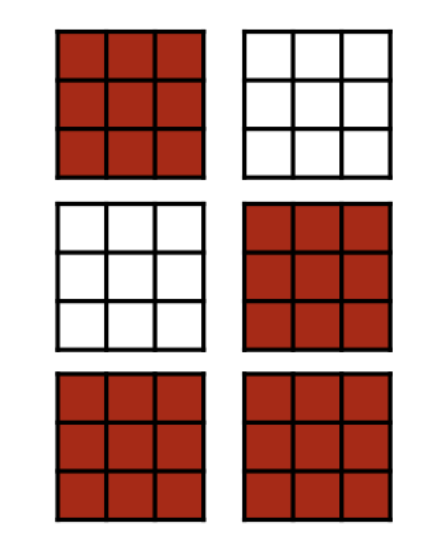
\includegraphics[width=0.2\linewidth]{report_images/kernel_pruning.png}
\caption{\label{fig:kernel_pruning_diag}Kernel Pruning}
\end{figure}

\noindent
We first take each kernel and calculate their frobenius norms.
\begin{equation}
||\mathbf{A}||_F = \sqrt{\sum_{i,j}a_{ij}^2}
\end{equation}
Now provided a sparsity value $s\%$ for a particular layer, $s\%$ of kernels with lower frobenius norms are pruned.
\begin{equation}
\textnormal{Importance}=||\mathbf{W}_k||_F
\end{equation}
where, $\mathbf{W}_k$ is a kernel of a particular layer. 

\subsection{Filter}
Filter pruning takes a more holistic approach by evaluating and eliminating entire filters from convolutional layers. This method 
not only prunes weights but also reduces the overall depth of the model. 

\begin{figure}[h]
\centering
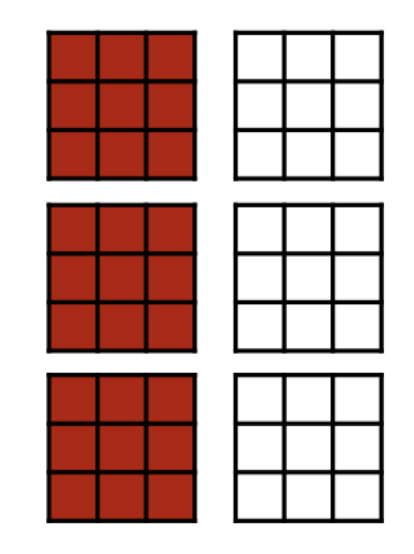
\includegraphics[width=0.2\linewidth]{report_images/filter_pruning.png}
\caption{\label{fig:filter_pruning_diag}Filter Pruning}
\end{figure}

\noindent
Since filters are tensors, we first take each filter and unroll them to a 2-D matrix. We then calculate the frobenius norms of each of these matrices and prune them based on the magnitudes of their norms.
\begin{equation}
\textnormal{Importance}=||\mathbf{W}_{\textnormal{flattened}}||_F
\end{equation}
where $||\mathbf{W}_{\textnormal{flattened}}||_F$ is the flattened 2-D matrix of a filter.

%%%%%%%%%%%%%%%%%%%%%%%%%%%%%%%%%%%%%%%%%%%%%%%
\section{Model}
\subsection{Architecture}

The architecture of the model used resembles a VGG-16 architecture with 4 convolutional blocks and a feed forward network as its head. In Fig~\ref{fig:conv_block}, each convolutional layer has a \textbf{kernel size} of $3\times3$, \textbf{stride} of $1$ and \textbf{padding} of $1$. 

\begin{figure}[h]
  \centering
  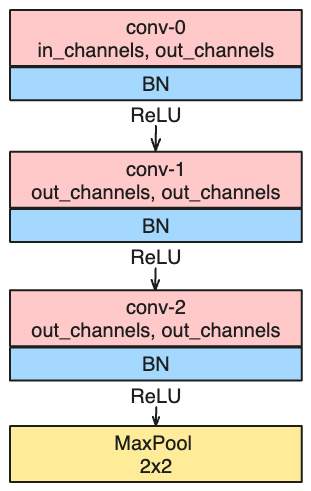
\includegraphics[width=0.25\linewidth]{report_images/conv_block.png}
  \caption{\label{fig:conv_block}A single convolutional block}
\end{figure}

\begin{figure}[h]
  \centering
  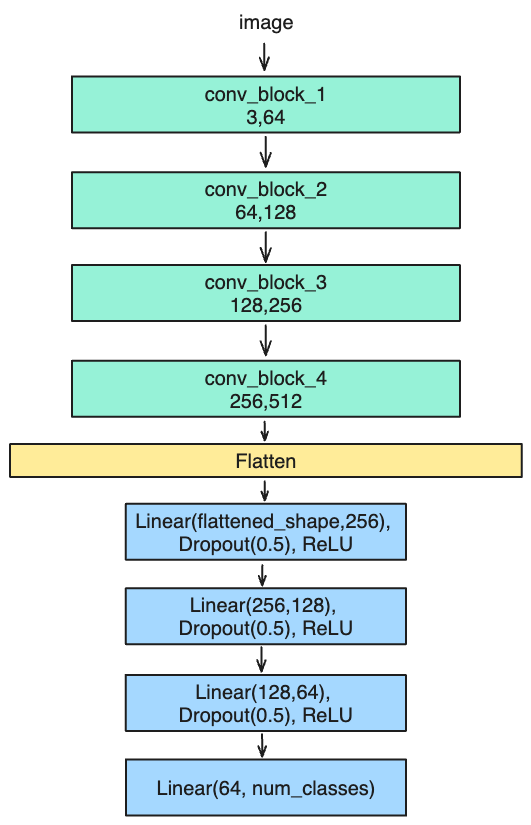
\includegraphics[width=0.4\linewidth]{report_images/architecture.png}
  \caption{\label{fig:architecture}CNN Architecture}
\end{figure}


All the convolutional layers in Fig~\ref{fig:architecture} are named from 'conv0 to 'conv11'. So there are a total of 12 convolutional layers.

\subsection{Hyper-parameters}
Some of the common hyper-parameters I used to train the un-pruned model and fine-tune the pruned ones are the following:
\begin{itemize}
\item Optimizer: \textbf{Adam} with default Pytorch settings except for the learning rate.
\item Learning Rate = 0.0001
\item Number of Parameters = 8,391,882
\item Batch Size = 64
\end{itemize}

\noindent
I trained the \textbf{un-pruned model} for \textbf{100 epochs} while the \textbf{pruned models} were fine-tuned for \textbf{20 epochs} each. 

%%%%%%%%%%%%%%%%%%%%%%%%%%%%%%%%%%%%%%%%%%%%%%%
\section{Sensitivity Scanning}
Sensitivity scanning refers to a systematic approach for identifying how sensitive different layers or components of a neural network are to pruning. The primary goal of sensitivity scanning is to determine which weights, neurons, or layers can be removed with minimal impact on the model's performance.
\subsection{Implementation}
For each pruning technique, I iterate over the weight tensor of each convolutional layer, prune them with sparsity values ranging from 0 to 0.9 with a step size of 0.1 and plot the accuracy of each instance of pruning.
\subsection{Results}
\begin{figure}[h]
  \centering
  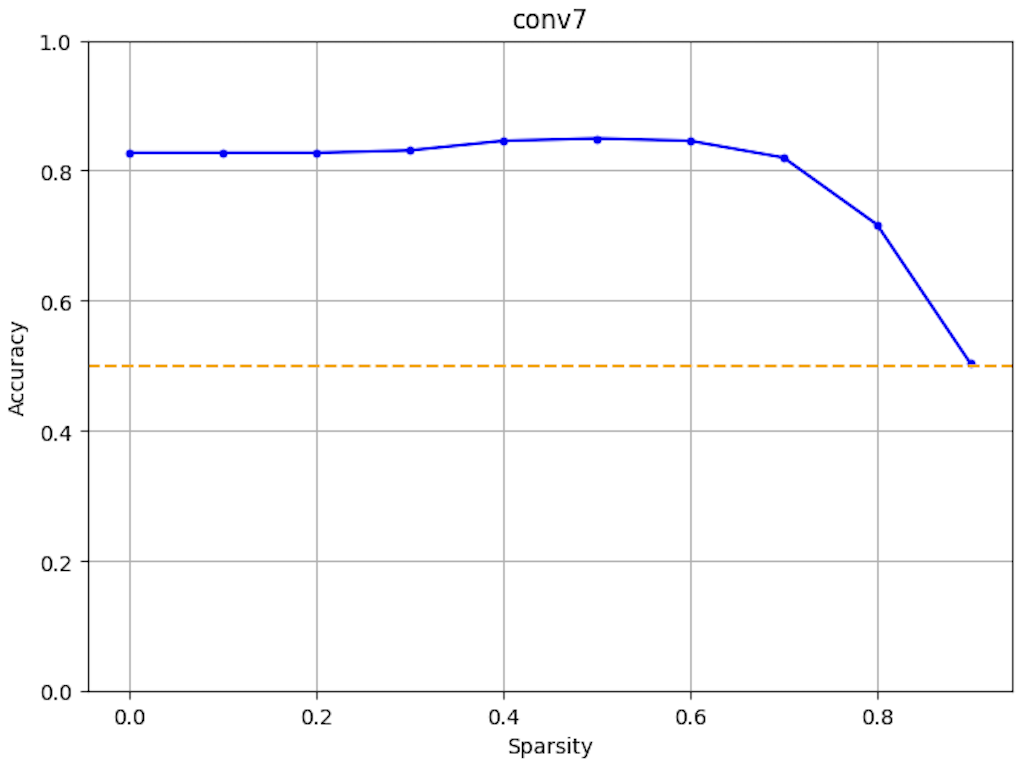
\includegraphics[width=0.4\linewidth]{report_images/fine_sense_egs.png}
  \caption{\label{fig:fine_sense_egs}Sensitivity Scan}
\end{figure}
\noindent
For all the sensitivity scans, we can see that the initial convolutional layers are more important than the latter ones even though they have significantly lesser parameters (Fig \ref{fig:fine_change_egs}). In some instances the accuracy doesn't even budge before the 0.7 or 0.8 range while pruning these deeper layers (Fig \ref{fig:fine_no_change_egs}). All graphs are in Section \ref{graphs_section}.

\begin{figure}[h]
\centering
\begin{minipage}{.4\textwidth}
  \centering
  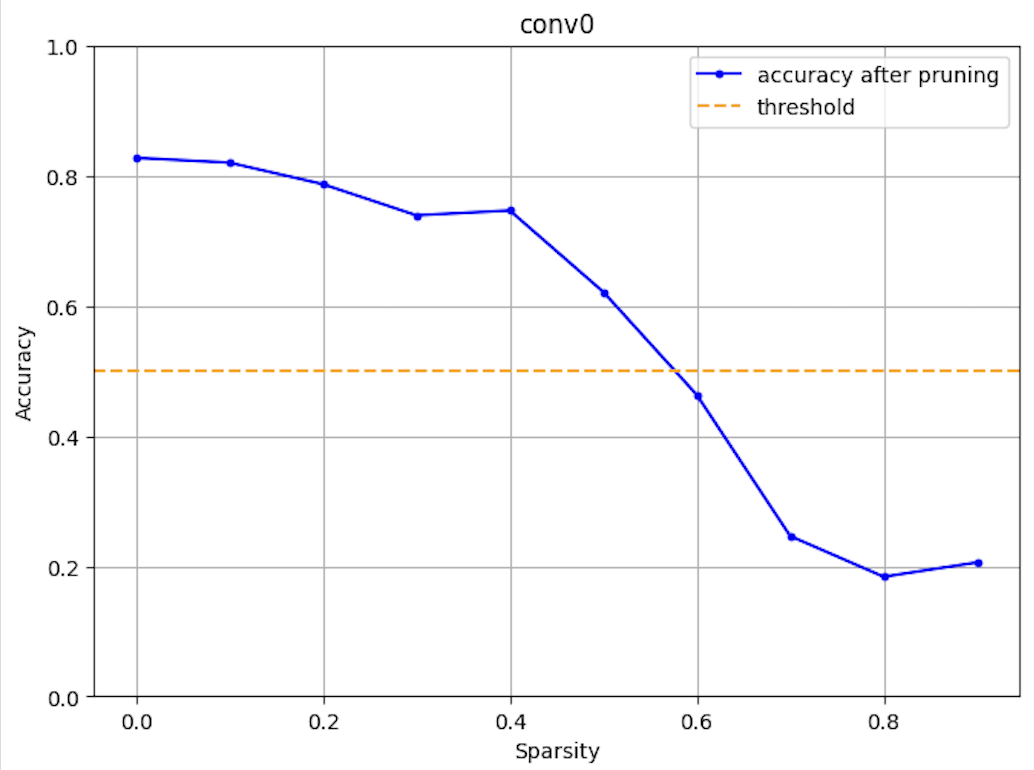
\includegraphics[width=1\linewidth]{report_images/fine_change_egs.png}
  \caption{Sensitivity Scan of an Earlier Layer}
  \label{fig:fine_change_egs}
\end{minipage}
\hspace{1.5 cm}
\begin{minipage}{.4\textwidth}
  \centering
  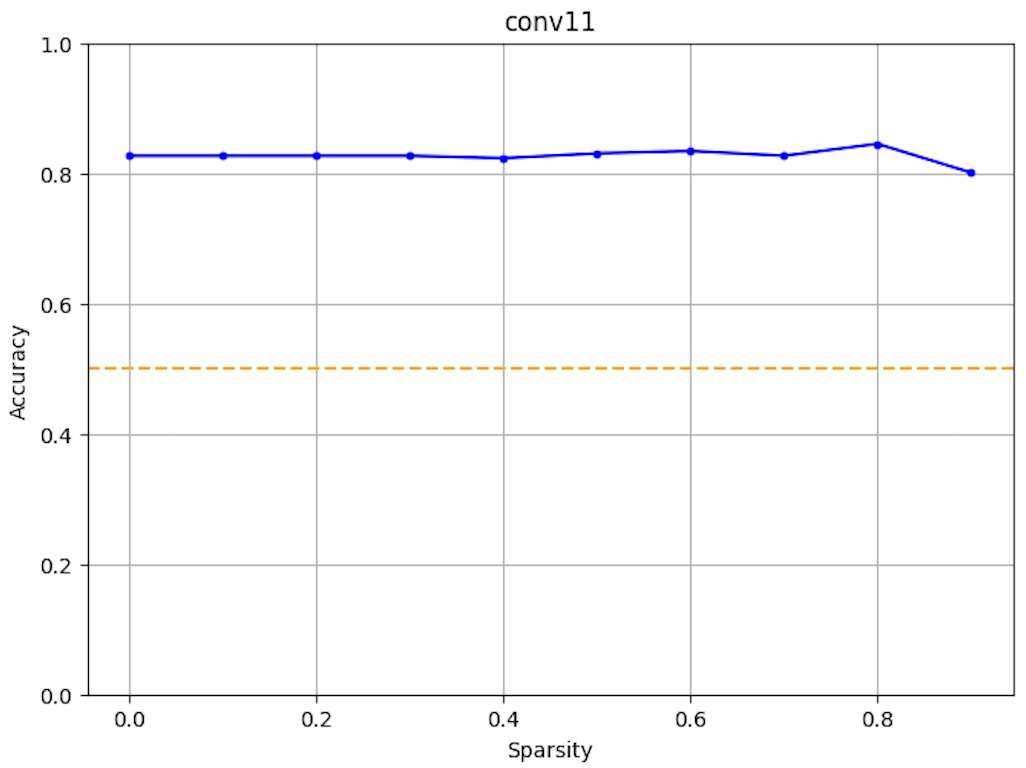
\includegraphics[width=1\linewidth]{report_images/fine_no_change_egs.png}
  \caption{Sensitivity Scan of a Deeper Layer}
  \label{fig:fine_no_change_egs}
\end{minipage}%
\end{figure}

\noindent
The first few layers are responsible for capturing low level features that are important for subsequent layers to build upon. Pruning can lead to failure of detecting  key features which can drop accuracy significantly. 

Since the initial layers have lesser parameters, when pruned there are lesser parameters to compensate for the loss in performance.

The deeper layers may be over parametrised, meaning they have more parameters than necessary, hence leading to less loss of performance when pruned. 

Also note that for some layers, the accuracy increases when its pruned. This could be due to the fact that the more the model we prune, the more it is able to generalise (I am plotting accuracy of these pruned models on the test dataset). 

%%%%%%%%%%%%%%%%%%%%%%%%%%%%%%%%%%%%%%%%%%%%%%%
\section{Pruning Heuristic}
After performing the sensitivity scans and going over the graphs, I decided to assign a \textbf{sparsity value} to each layer just before they dipped below the \textbf{50\% accuracy mark}. The sparsity levels are displayed in Table \ref{tab:pruning_levels}.
\begin{table}[h]
\centering
\begin{tabular}{lccc}
\hline
\textbf{Layer} & \textbf{Fine-grained} & \textbf{Kernel} & \textbf{Filter} \\
\hline
conv0  & 0.5 & 0.3 & 0.4 \\
conv1  & 0.8 & 0.6 & 0.3 \\
conv2  & 0.7 & 0.3 & 0.3 \\
conv3  & 0.7 & 0.5 & 0.3 \\
conv4  & 0.7 & 0.5 & 0.2 \\
conv5  & 0.8 & 0.7 & 0.4 \\
conv6  & 0.7 & 0.6 & 0.2 \\
conv7  & 0.8 & 0.6 & 0.4 \\
conv8  & 0.8 & 0.7 & 0.6 \\
conv9  & 0.8 & 0.8 & 0.5 \\
conv10 & 0.9 & 0.9 & 0.6 \\
conv11 & 0.9 & 0.9 & 0.9 \\
\hline
\end{tabular}
\caption{\label{tab:pruning_levels}Sparsity Levels for Different Pruning Methods}
\end{table}

\section{Results}
As discussed before I trained the \textbf{un-pruned model} for \textbf{100 epochs} while the \textbf{pruned models} were fine-tuned for \textbf{20 epochs} each. 

The \textbf{accuracy} of the \textbf{un-pruned model} on the test dataset is $\boldsymbol{85.03\%}$. 

\begin{table}[h]
\centering
\label{tab:vgg16_pruning_impact}
\begin{tabular}{|p{3.25cm}||p{3.25cm}|p{3.25cm}|p{3.25cm}|}
\hline
\textbf{Strategy} & \textbf{\% Parameters  Remaining} & \textbf{Accuracy After Pruning(\%)} & \textbf{Accuracy After Fine-tuning(\%)} \\
\hline
Fine-grained & 20.4959 & \textbf{40.81} & \textbf{82.69} \\
Kernel & 23.9542 & 17.94 & 80.70 \\
Filter & 41.4917 & 14.05 & 82.44 \\
\hline
\end{tabular}
\caption{Impact of Pruning Strategies on Model}
\end{table}
\noindent
\textbf{Fine-grained pruning retains the most accuracy} after being applied while filter saw the most drop. 

Since fine-grained pruning operates at a granular level, it can often really narrow in on each individual weight and gauge their importance to the network. On the other hand, filter and kernel pruning removes entire tensors all at once which can lead to important feature detectors being removed. 

Fine-grained pruners are like expert sculptors, having justified intention to chisel away each flake of wood to perfect his creation while kernel and filter pruners are amateurs sculptors making broader strokes, that may shape the figure quickly but risk losing some finer, nuanced detail.

Although, the kernel and filter pruning strategies bring the down the accuracies by a significant margin, all three models are easily able to gain their performance back with proper fine-tuning.

%%%%%%%%%%%%%%%%%%%%%%%%%%%%%%%%%%%%%%%%%%%%%%%
\section{Weight Distributions}
I plotted the weights of all the convolutional layers of seven different variations of the model. The un-pruned model and models on which the three pruning strategies are applied, both before and after fine-tuning. All the distributions are in Section \ref{weight_distribution}.

\subsection{Un-pruned}
Fig \ref{fig:unpruned_w_dist} is the weight distribution of conv7 of the trained model.
\begin{figure}[h]
  \centering
  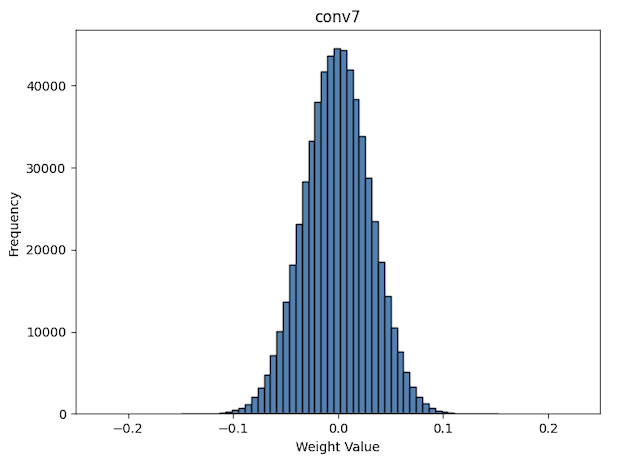
\includegraphics[width=0.5\linewidth]{report_images/unpruned_w_dist.png}
  \caption{\label{fig:unpruned_w_dist}Distribution of Weights of a Layer in the Un-pruned Model}
\end{figure}

\subsection{Fine-grained Pruning}
Since fine-grained pruning involves pruning based on magnitude, we see that weights with values near zero being heavily filtered out. The 'conv7' layer for fine-grained pruning has a sparsity value of 0.8, so there is a significant decrease in number of weights as well. (Fig \ref{fig:fine_w_dis})

\begin{figure}[h]
\centering
\begin{subfigure}{.5\textwidth}
  \centering
  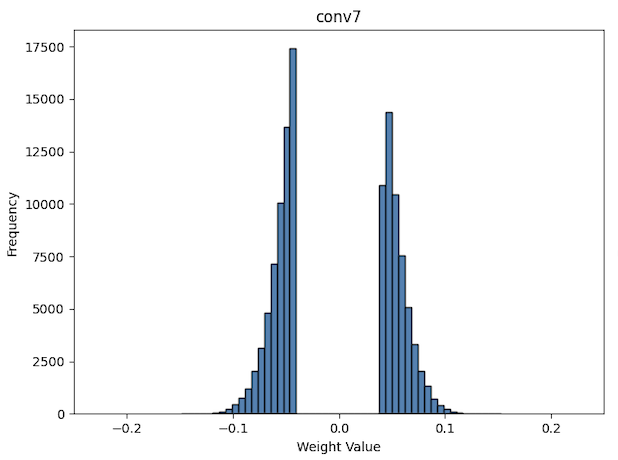
\includegraphics[width=1\linewidth]{report_images/finegrained_w_dist_pp.png}
  \caption{Pre-Fine-tuning}
  \label{fig:fine_dis_tt}
\end{subfigure}%
\begin{subfigure}{.5\textwidth}
  \centering
  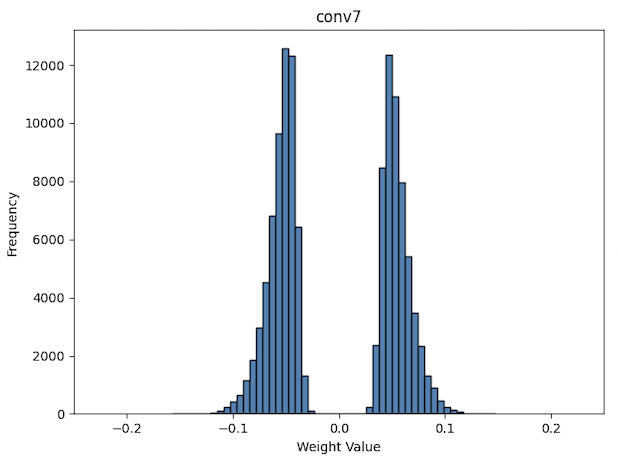
\includegraphics[width=1\linewidth]{report_images/finegrained_w_dist_ft.png}
  \caption{Post-Fine-tuning}
  \label{fig:fine_dis_ft}
\end{subfigure}
\caption{Fine-grained Pruning Weight Distribution}
\label{fig:fine_w_dis}
\end{figure}
\noindent
The distribution of the pre-fine-tuned weights have high bias due to most of the values near zero being removed. When we fine-tune, the weights gain some variance to compensate for learning capacity but never matches the distribution of the un-pruned  model.


\subsection{Kernel Pruning}
After kernel pruning, the tail ends of the distribution tends to gain some variance in its weights alluding to the fact that weights closer to zero have been removed but not as aggressively as fine-grained pruning. (Fig \ref{fig:kernel_w_dis})

Fine-tuning doesn't change the distribution much. It just re-purposes existing weights to fit the task. 


\begin{figure}[h]
\centering
\begin{subfigure}{.5\textwidth}
  \centering
  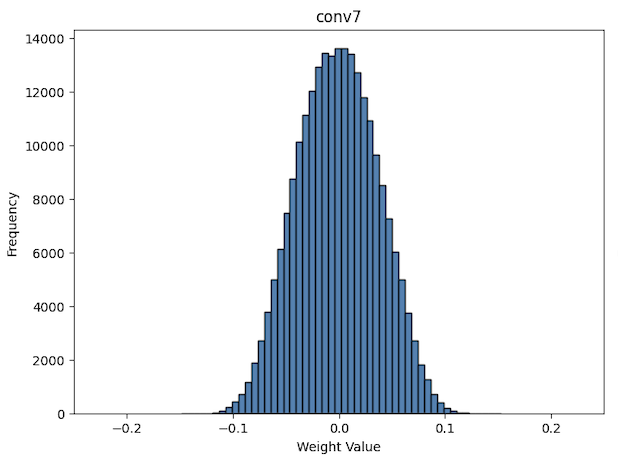
\includegraphics[width=1\linewidth]{report_images/kernel_w_dist_pp.png}
  \caption{Before Fine-tuning}
  \label{fig:kernel_dis_tt}
\end{subfigure}%
\begin{subfigure}{.5\textwidth}
  \centering
  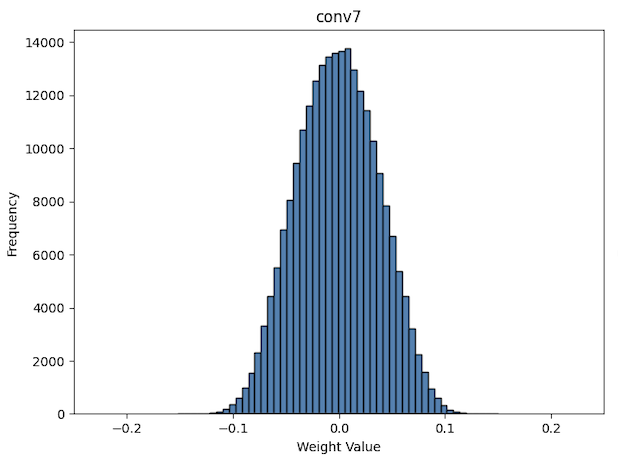
\includegraphics[width=1\linewidth]{report_images/kernel_w_dist_ft.png}
  \caption{After Fine-tuning}
  \label{fig:kernel_dis_ft}
\end{subfigure}
\caption{Kernel Pruning Weight Distribution}
\label{fig:kernel_w_dis}
\end{figure}


\subsection{Filter Pruning}
Distribution of weights remains the most constant with the original distribution. Since we are using much larger heuristic to prune weights, the number of weights actually closer to zero becomes significantly lower. Hence, very little change to the distribution. (Fig \ref{fig:filter_w_dis})


\begin{figure}[h]
\centering
\begin{subfigure}{.5\textwidth}
  \centering
  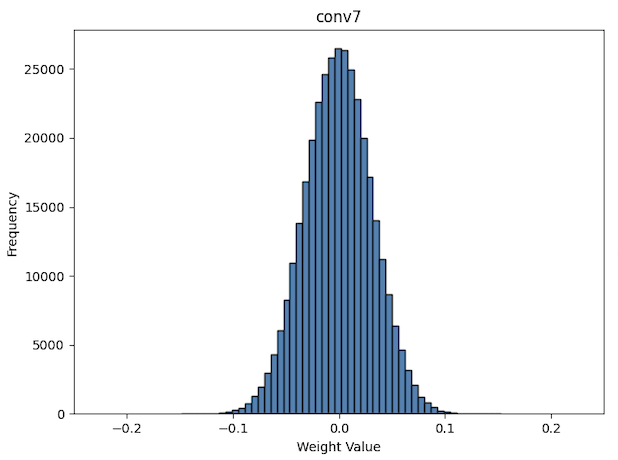
\includegraphics[width=1\linewidth]{report_images/filter_w_dist_pp.png}
  \caption{Before Fine-tuning}
  \label{fig:filter_dis_tt}
\end{subfigure}%
\begin{subfigure}{.5\textwidth}
  \centering
  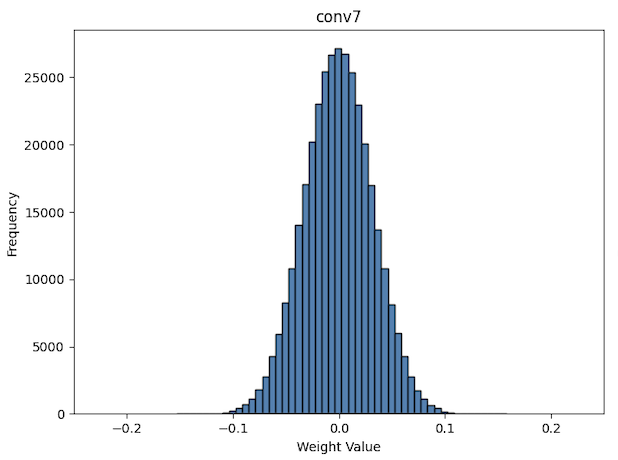
\includegraphics[width=1\linewidth]{report_images/filter_w_dist_ft.png}
  \caption{After Fine-tuning}
  \label{fig:filter_dis_ft}
\end{subfigure}
\caption{Filter Pruning Weight Distribution}
\label{fig:filter_w_dis}
\end{figure}
\FloatBarrier

%%%%%%%%%%%%%%%%%%%%%%%%%%%%%%%%%%%%%%%%%%%%%%%
\section{Activation Balances}

I passed Fig \ref{fig:Input_Image} into all the models and plotted a histogram of the activations. I pruned all the activations that equalled zero for each layer. All the distributions are in Section \ref{activations}.

\begin{figure}[h]
  \centering
  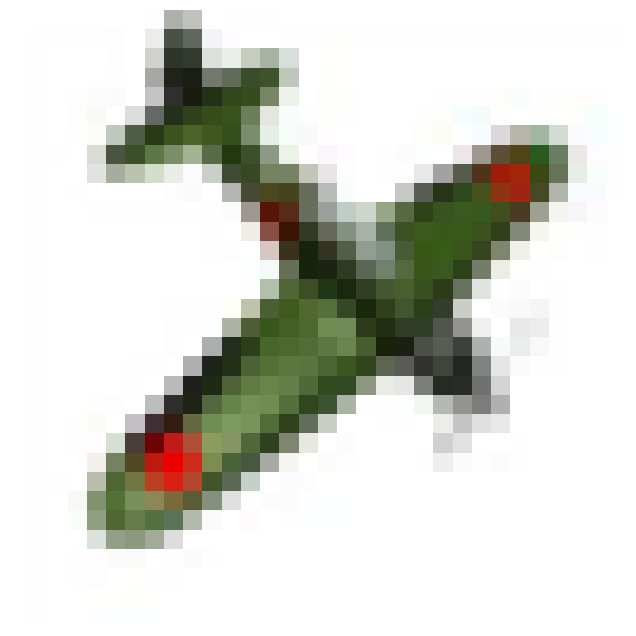
\includegraphics[width=0.4\linewidth]{report_images/plane_input.png}
  \caption{\label{fig:Input_Image}Input Image to the Models}
\end{figure}

%%%%%%%%%%%%%%%%%%%%%%%%%%%%%%%%%%%%%%%%%%%%%%%
\section{Conclusion}
We can see most performance being perserved by fine-grained pruning but its not much of a viable method because of how unstructured it is. GPUs can have hard time navigating through it. Kernel and channel pruning are quite structured and regain most of its performance in this report, but rigorous testing is required on how far can we go with them, how important the weights being pruned are, and whether using norms are a good method for these pruning strategy.

\pagebreak
%%%%%%%%%%%%%%%%%%%%%%%%%%%%%%%%%%%%%%%%%%%%%%%
\section{Appendix} 
\subsection{Sensitivity Scans}
\label{graphs_section}
\begin{figure}[h]
  \centering
  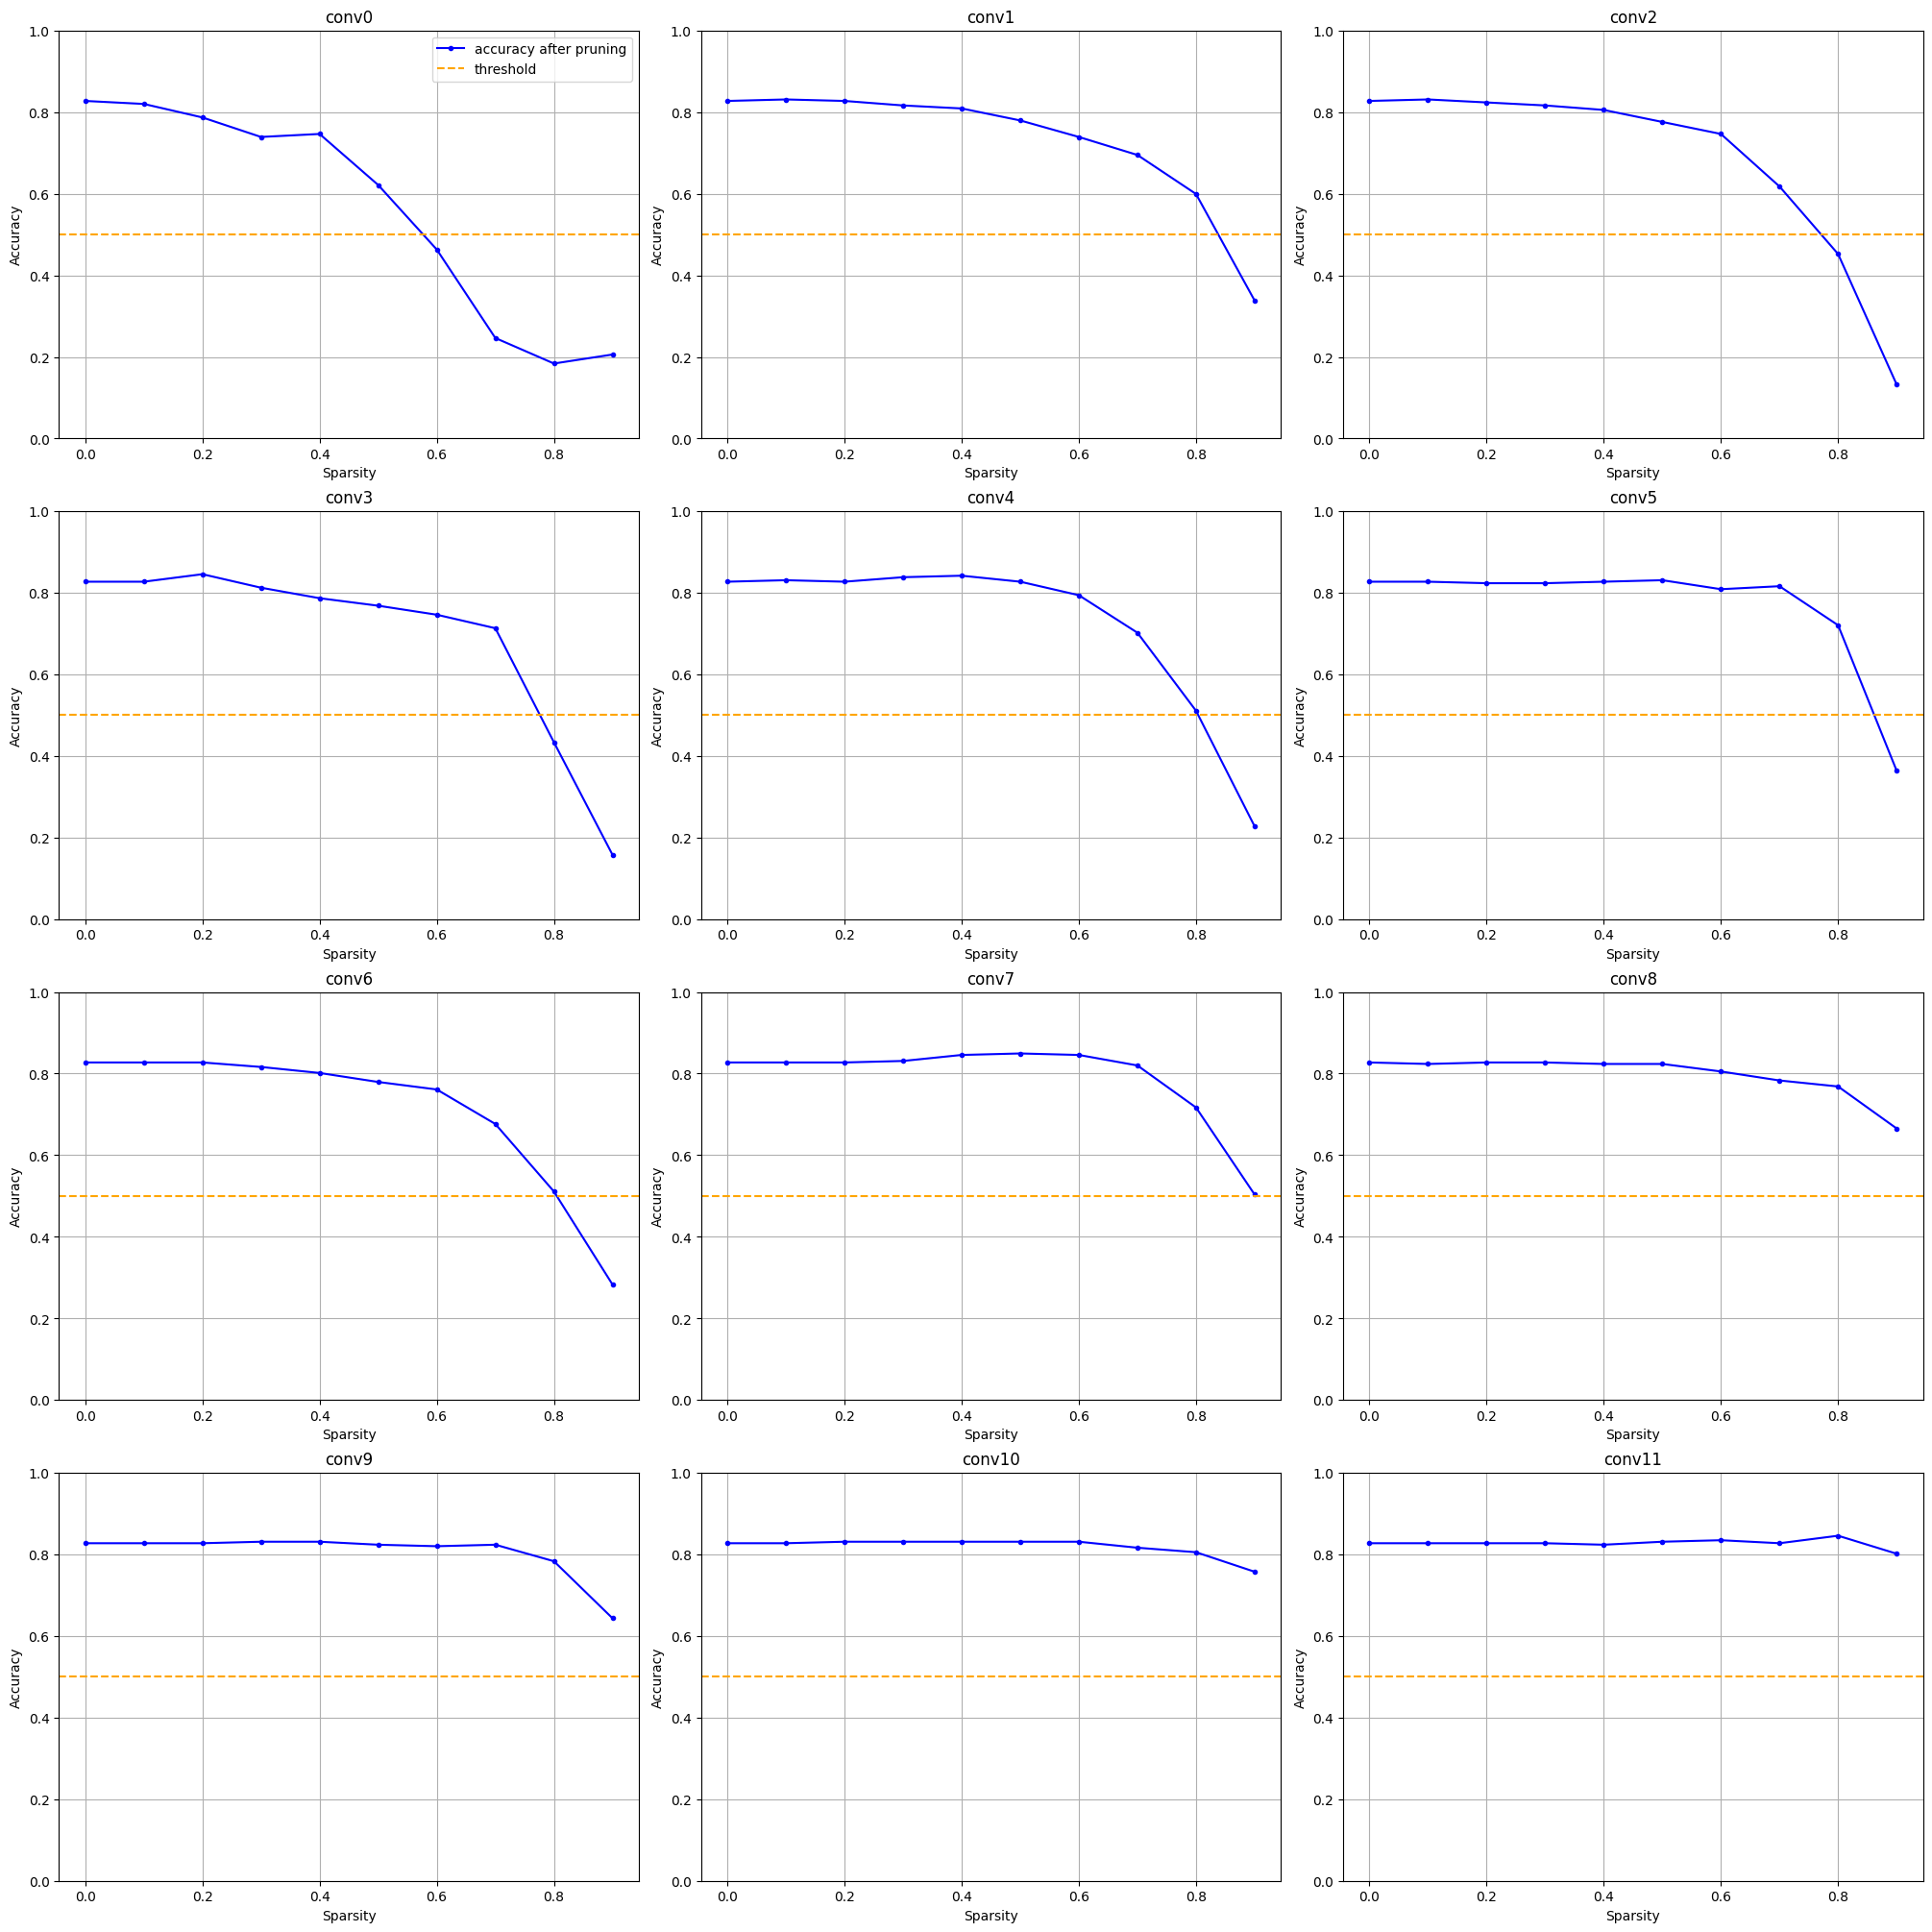
\includegraphics[width=1\linewidth]{report_images/sense_fine.png}
  \caption{\label{fig:sense_fine}Fine-grained Pruning Sensitivity Scan}
\end{figure}
\FloatBarrier

\begin{figure}[h]
  \centering
  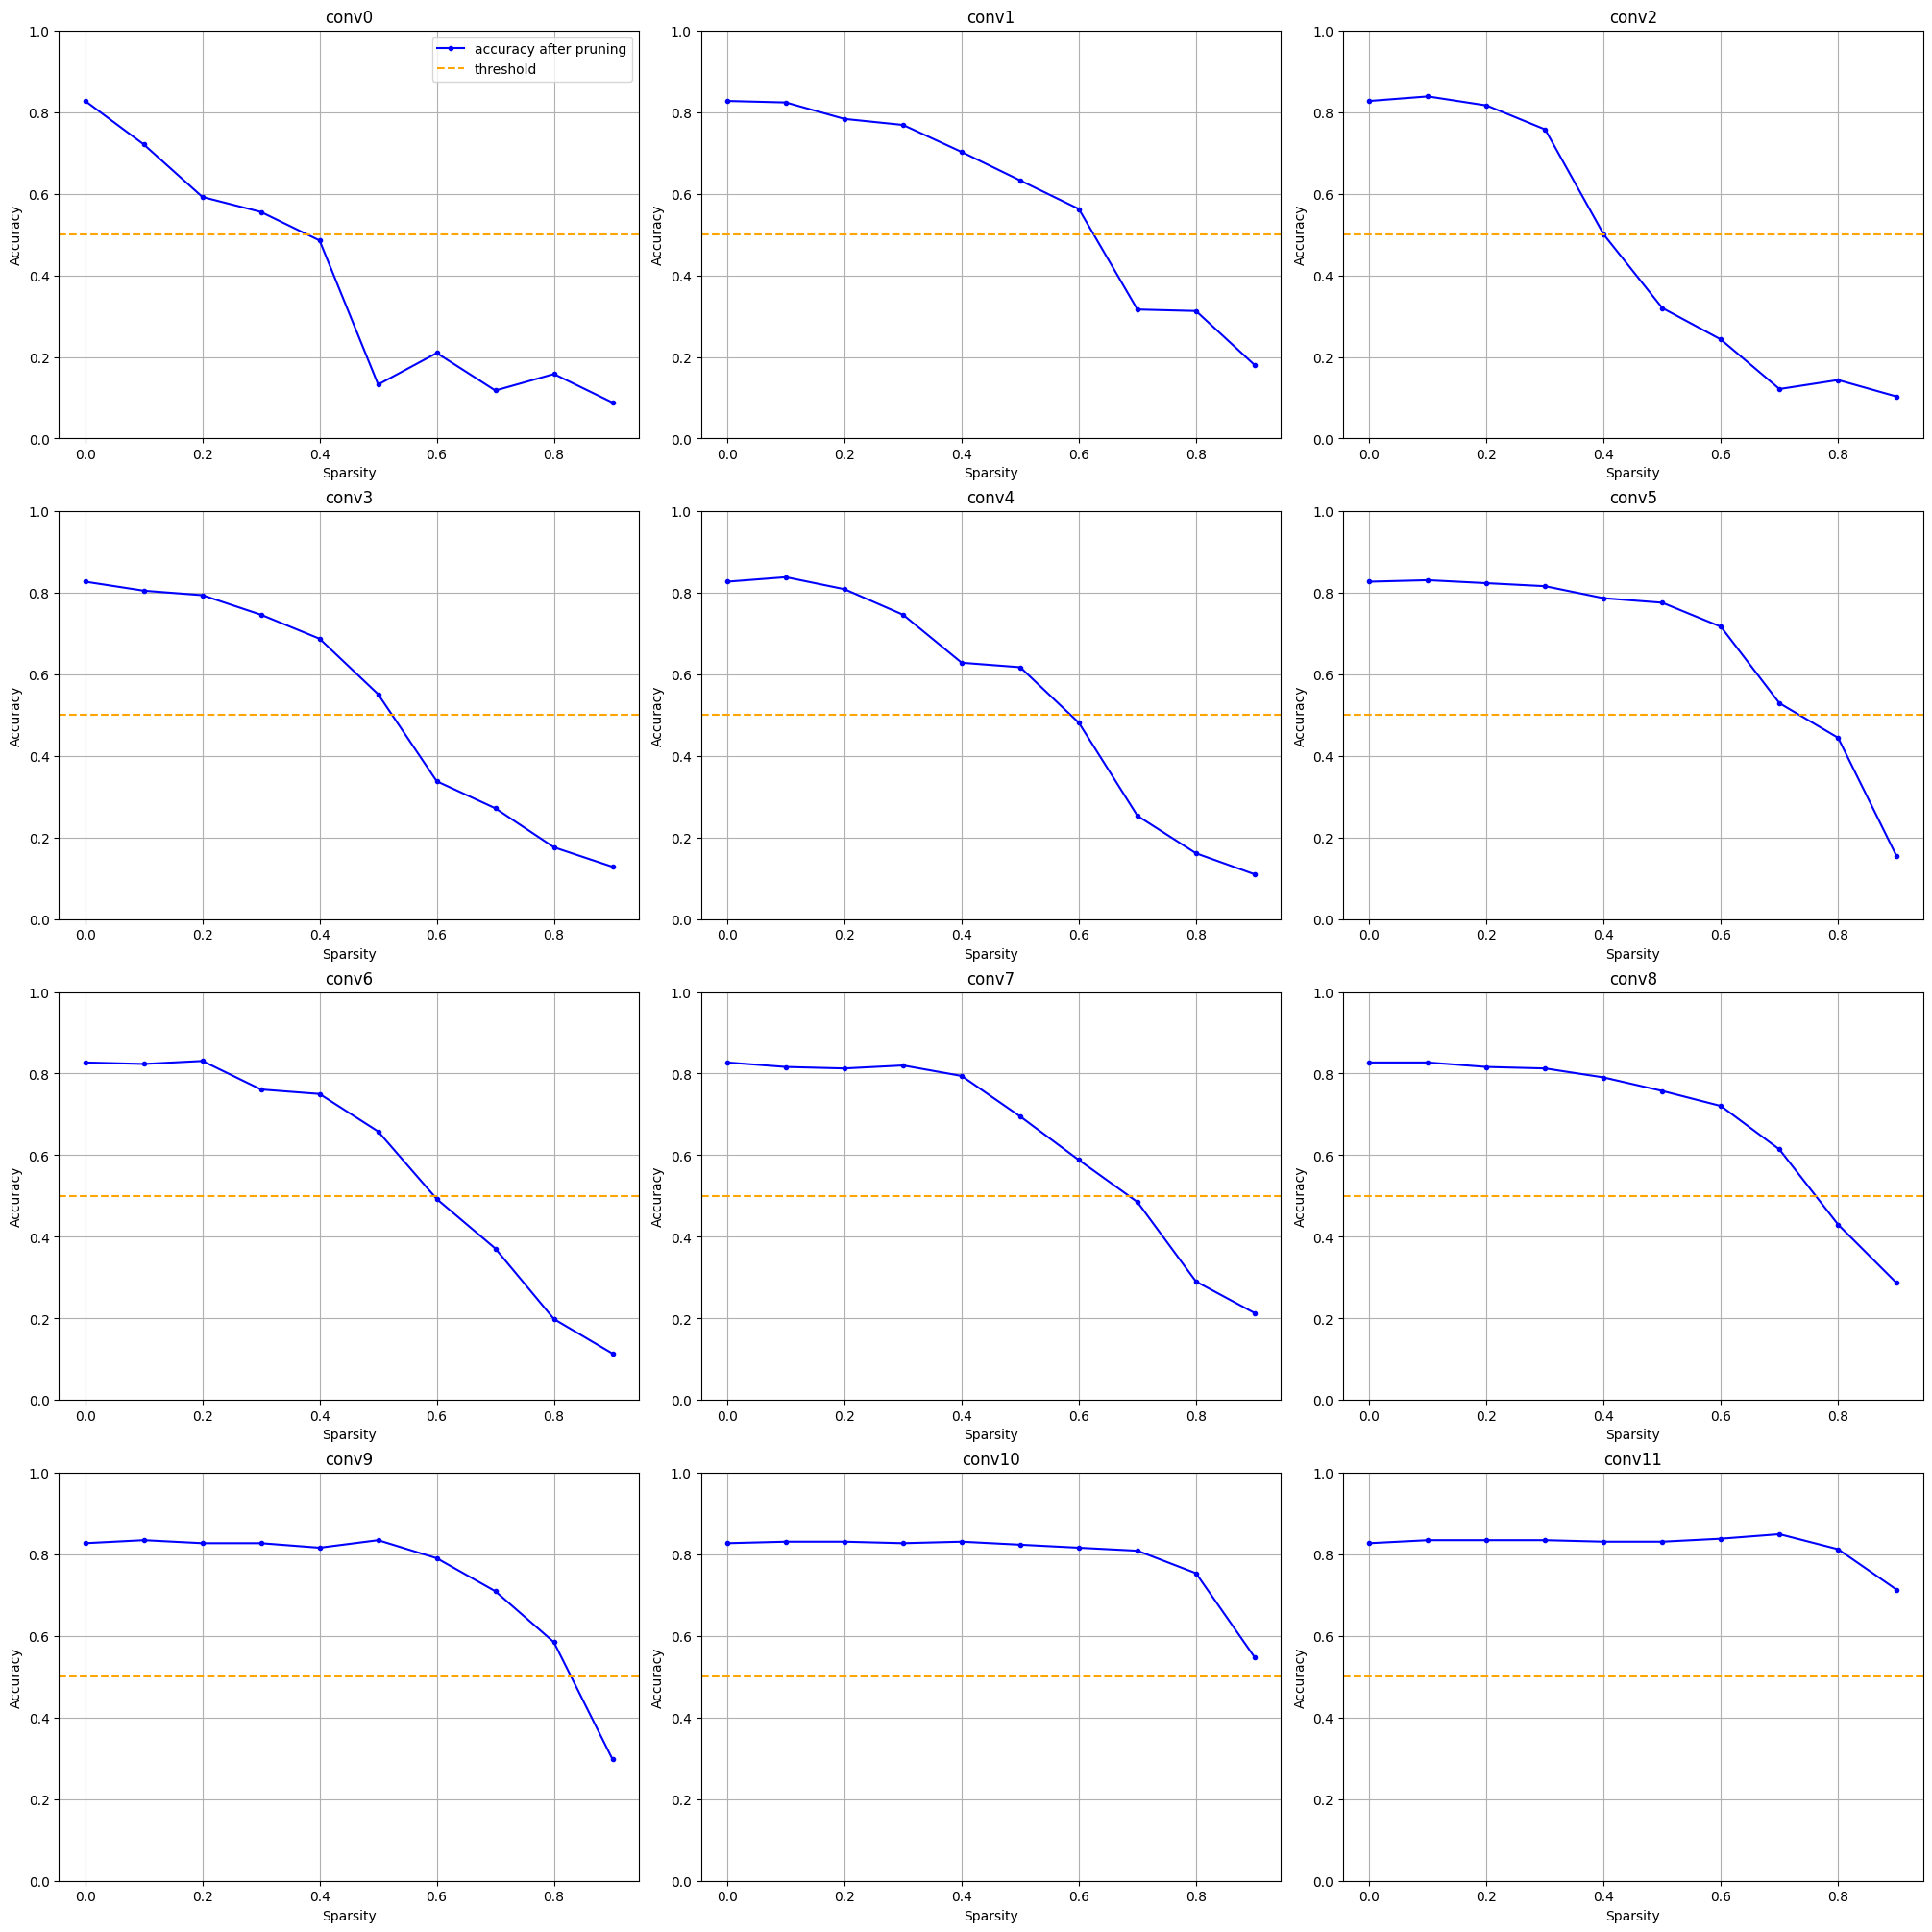
\includegraphics[width=1\linewidth]{report_images/sense_kernel.png}
  \caption{\label{fig:sense_kernel}Kernel Pruning Sensitivity Scan}
\end{figure}
\FloatBarrier

\begin{figure}[h]
  \centering
  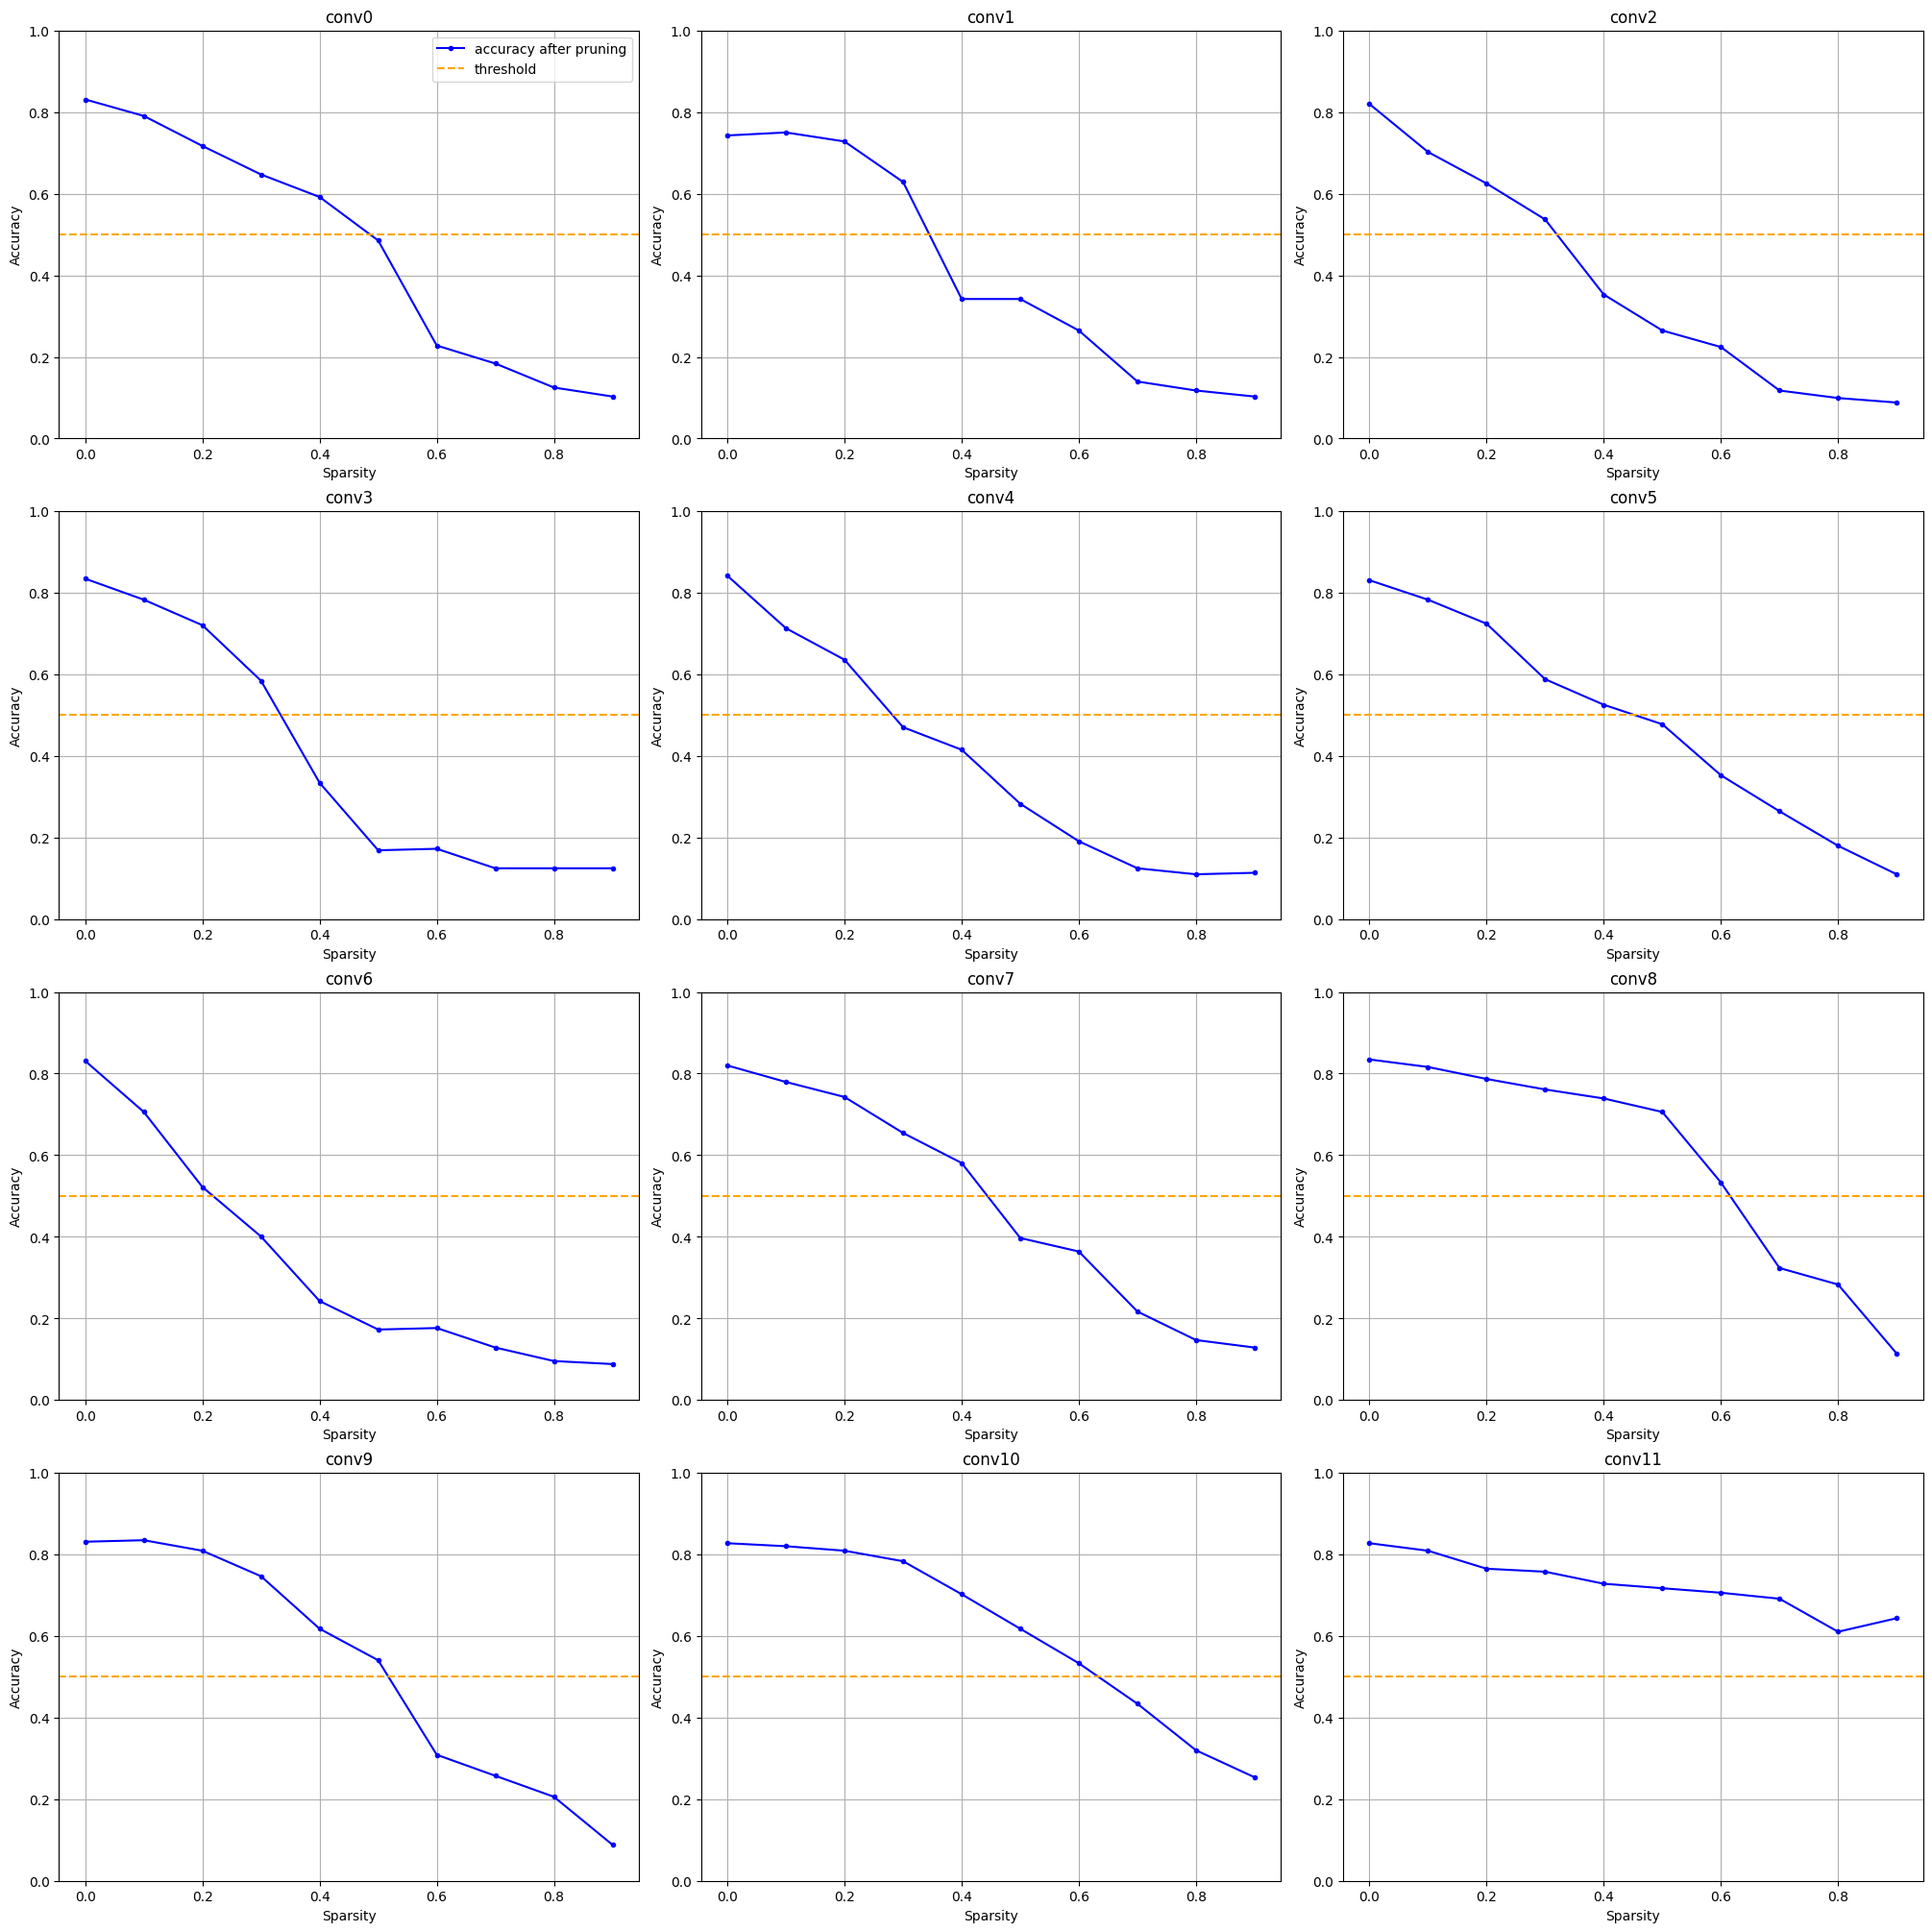
\includegraphics[width=1\linewidth]{report_images/sense_filter.png}
  \caption{\label{fig:sense_filter}Filter Pruning Sensitivity Scan}
\end{figure}
\FloatBarrier
\pagebreak

%%%%%%%
\subsection{Weight Distributions} 

\label{weight_distribution}
\begin{figure}[h]
  \centering
  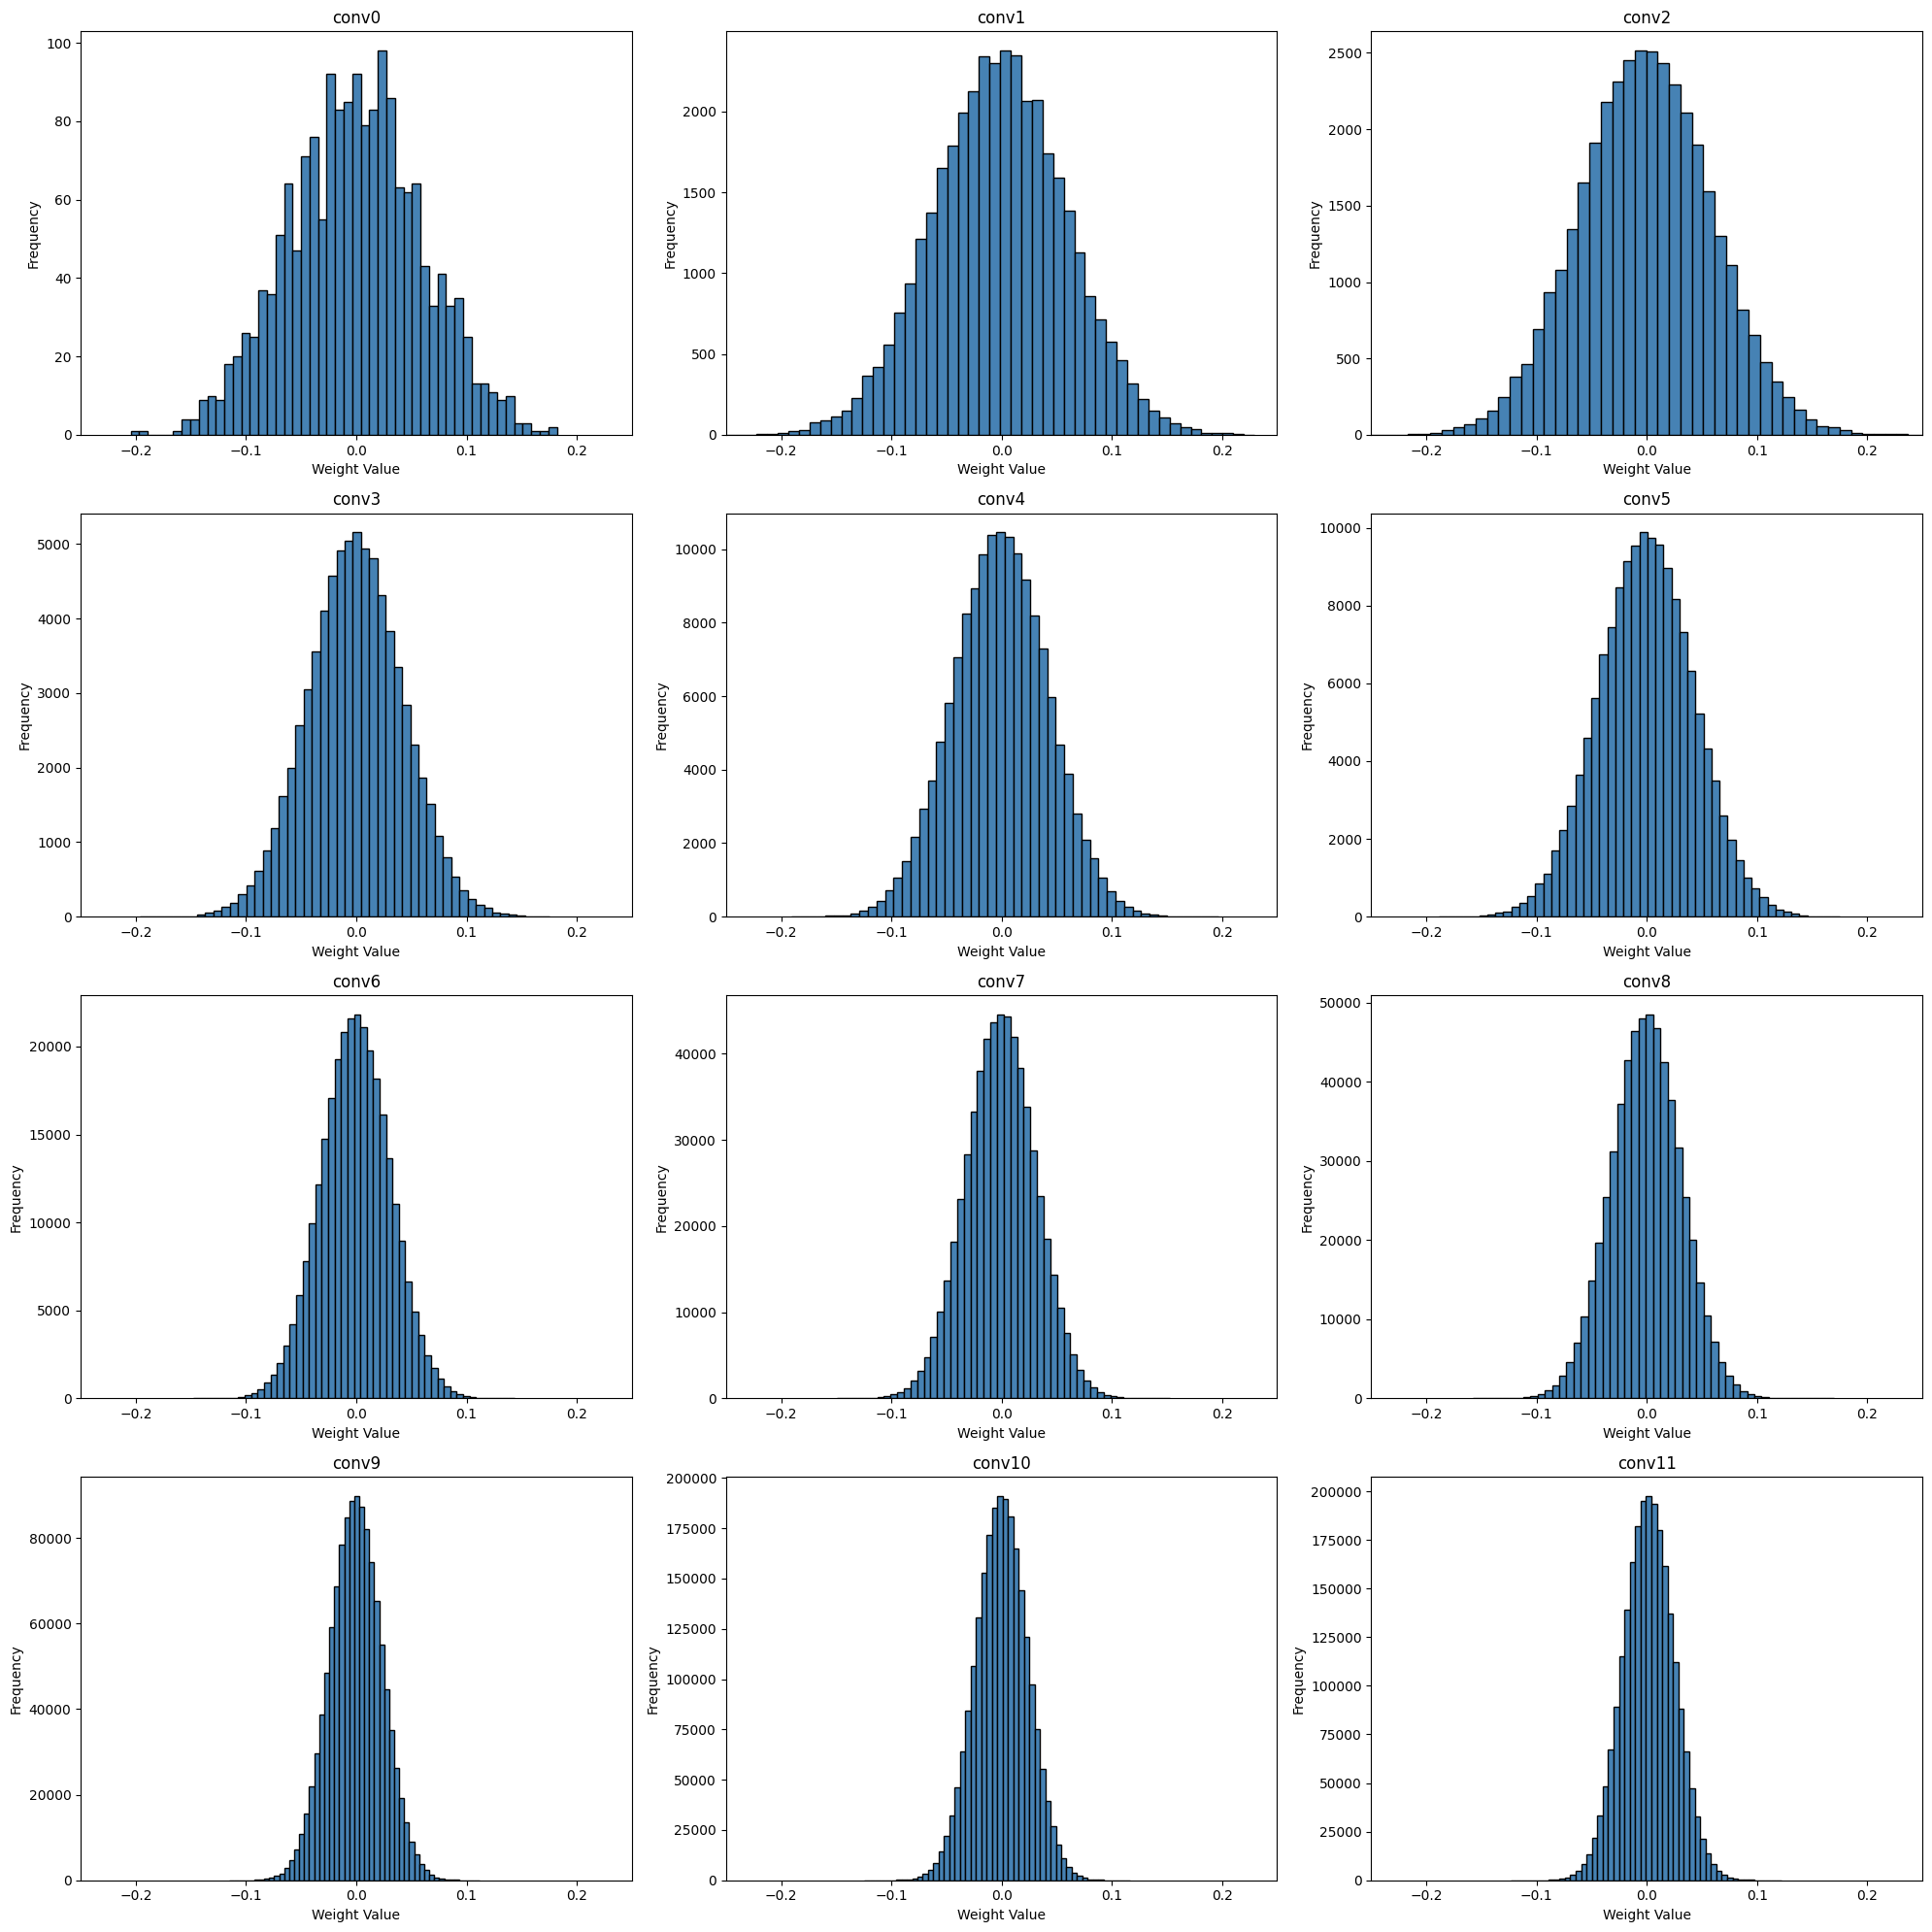
\includegraphics[width=1\linewidth]{report_images/unpruned_dist.png}
  \caption{\label{fig:unpruned_dist}Un-pruned Model Weights Distribution}
\end{figure}
\FloatBarrier

\begin{figure}[h]
  \centering
  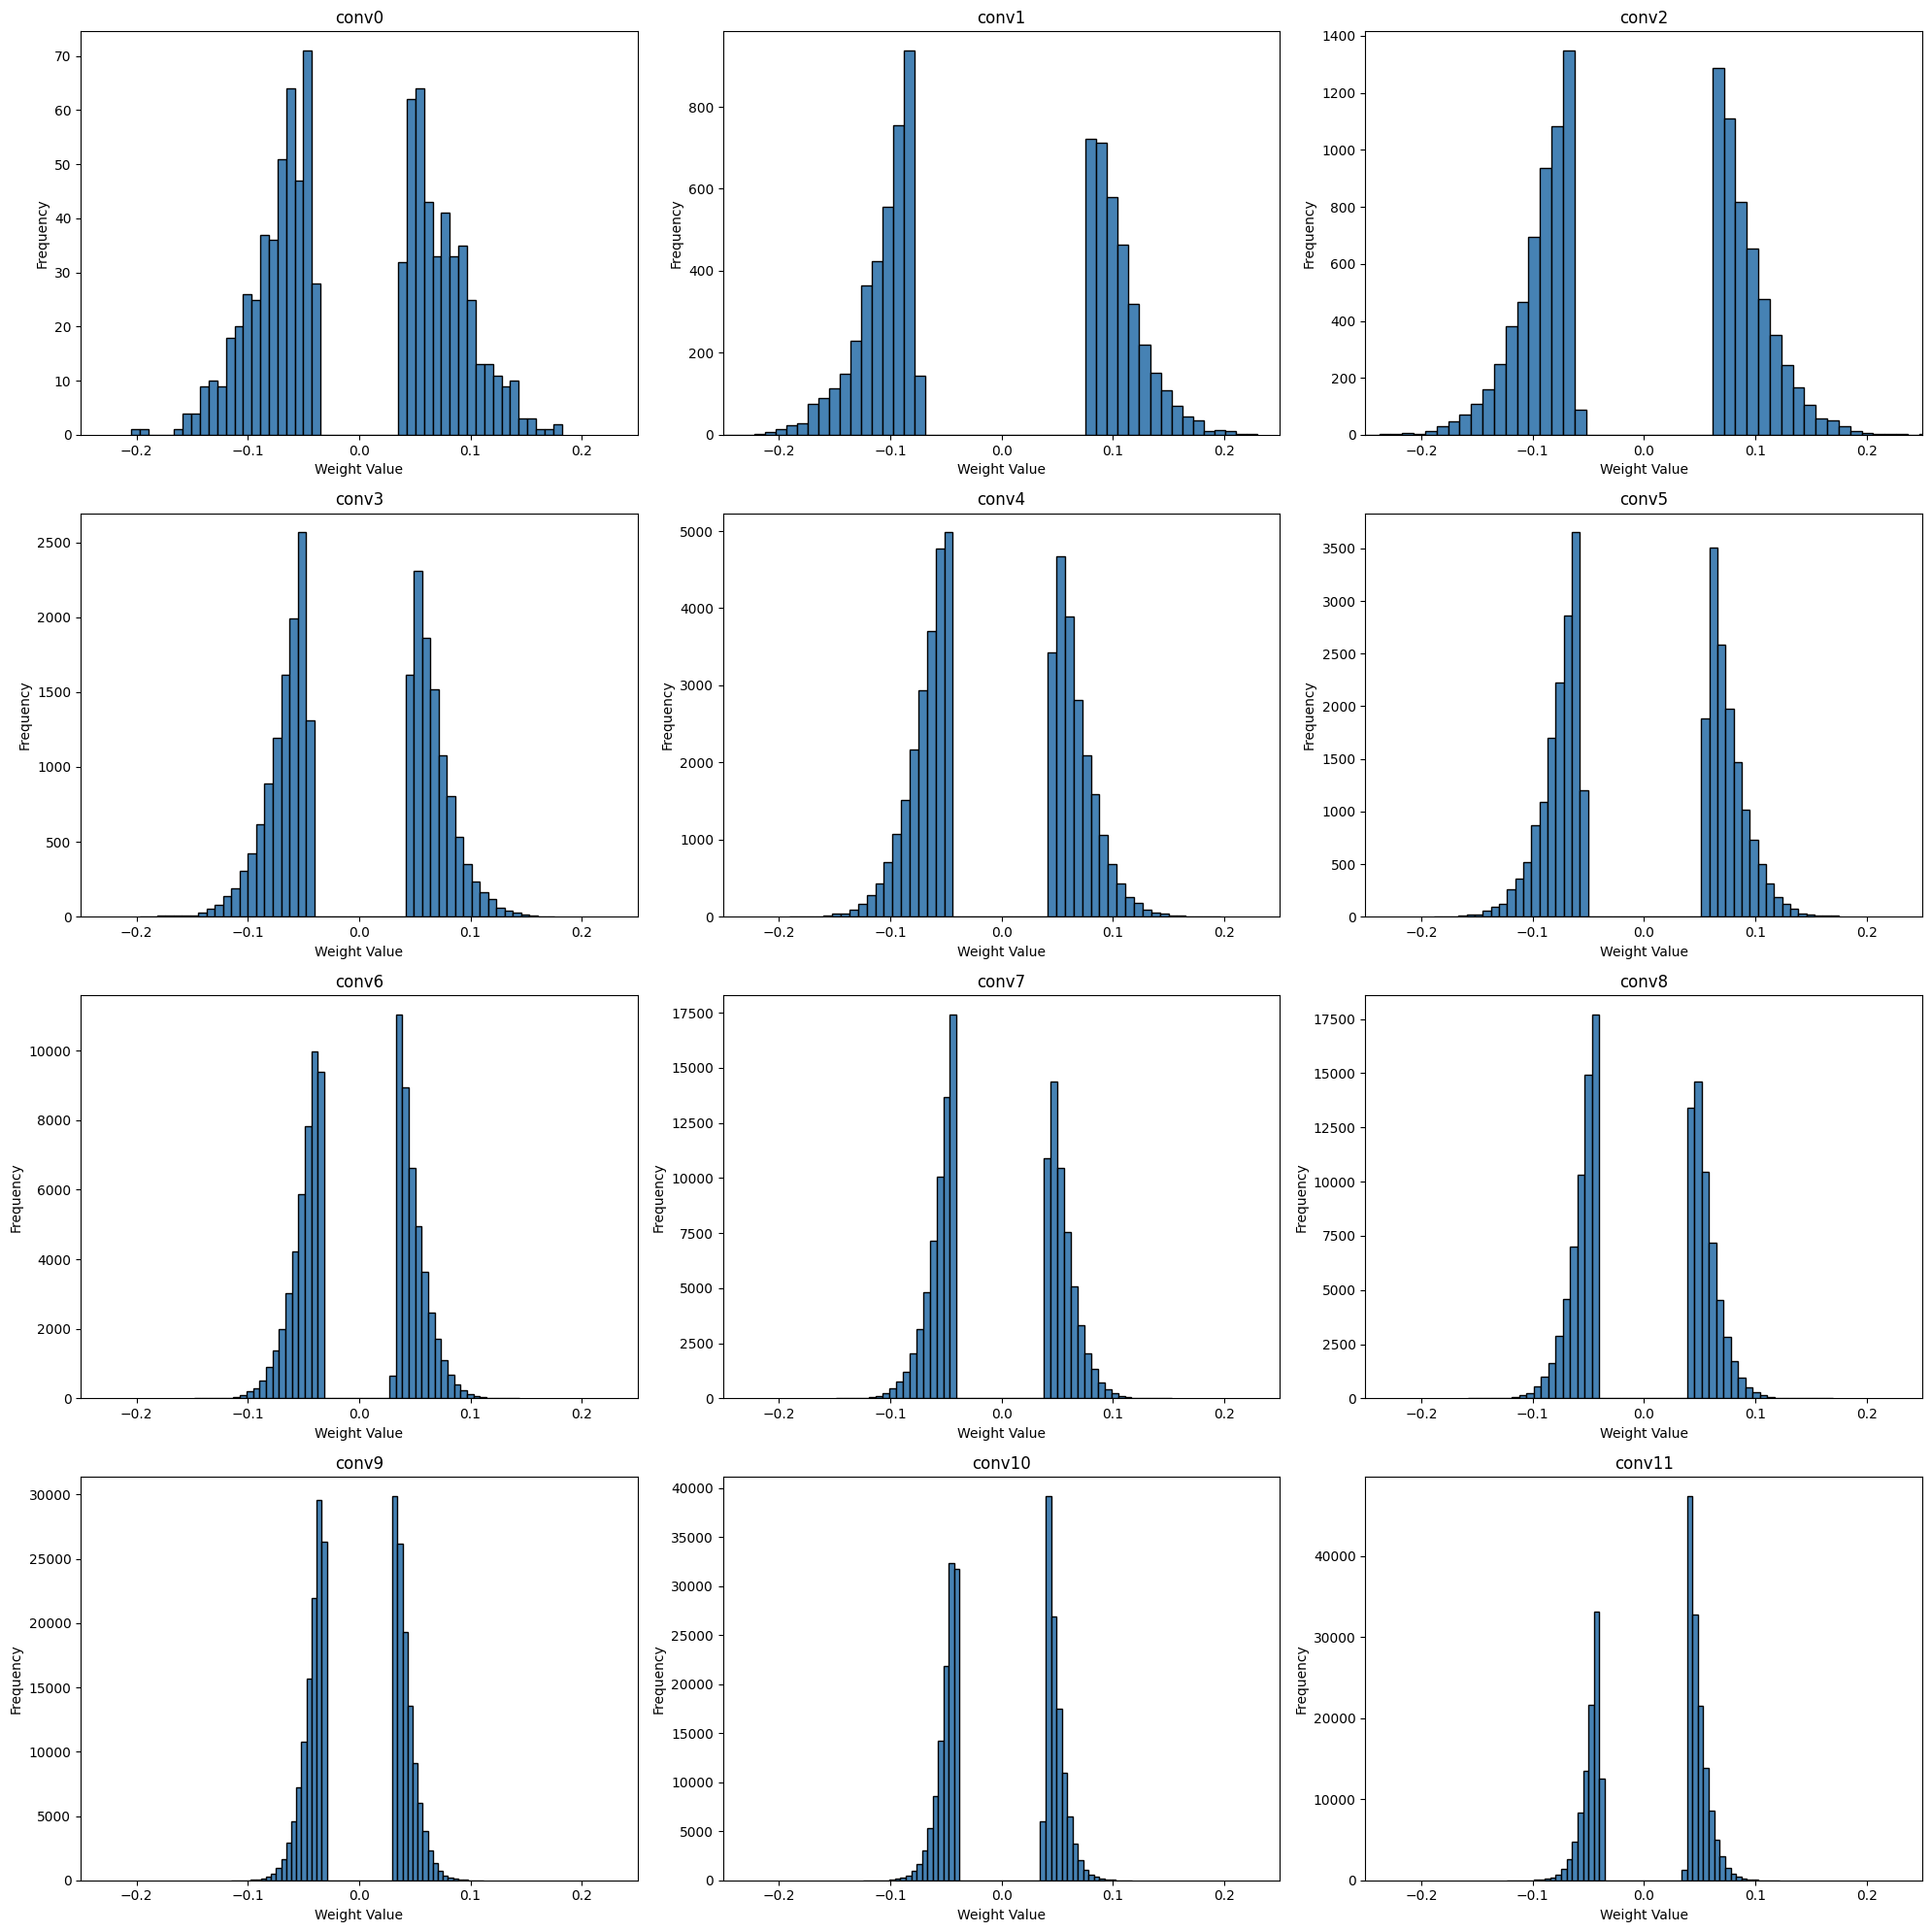
\includegraphics[width=1\linewidth]{report_images/fine_dist_pp.png}
  \caption{\label{fig:fine_dist_pp}Fine-grained Pruned Model Weights Distribution (Pre-Fine-tuning)}
\end{figure}
\FloatBarrier

\begin{figure}[h]
  \centering
  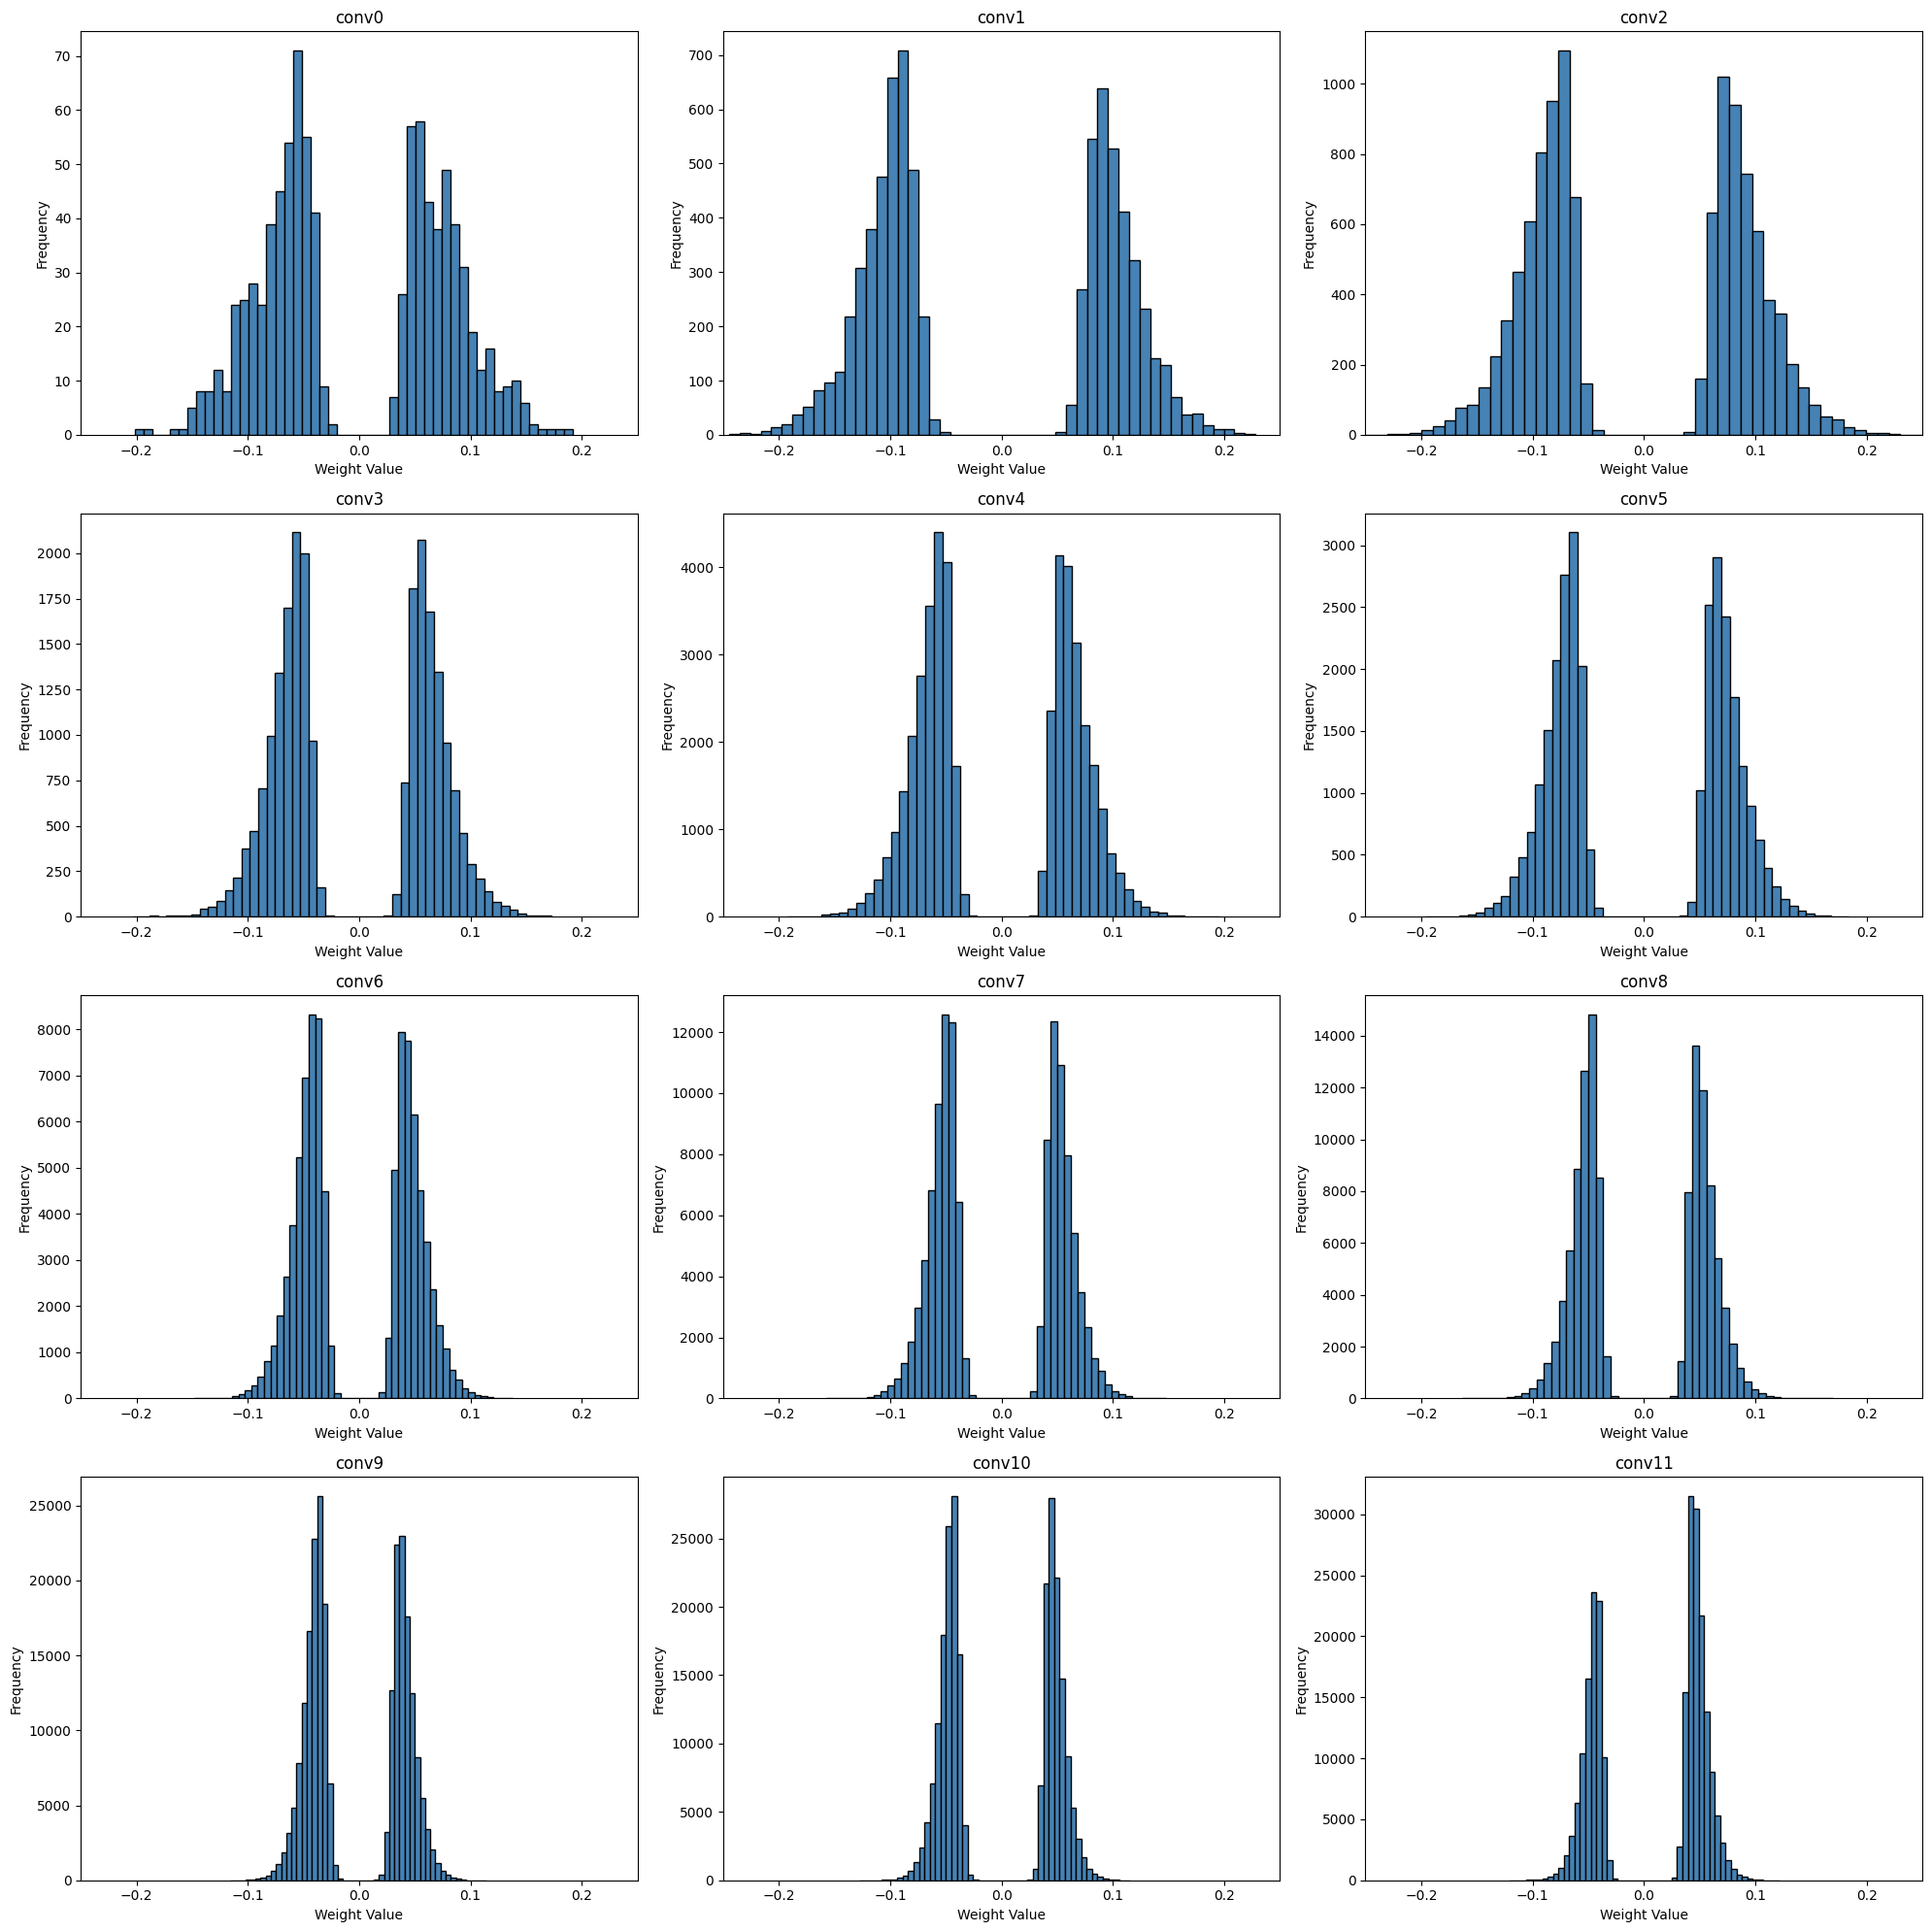
\includegraphics[width=1\linewidth]{report_images/fine_dist_ft.png}
  \caption{\label{fig:fine_dist_ft}Fine-grained Pruned Model Weights Distribution (Post-Fine-tuned)}
\end{figure}
\FloatBarrier

\begin{figure}[h]
  \centering
  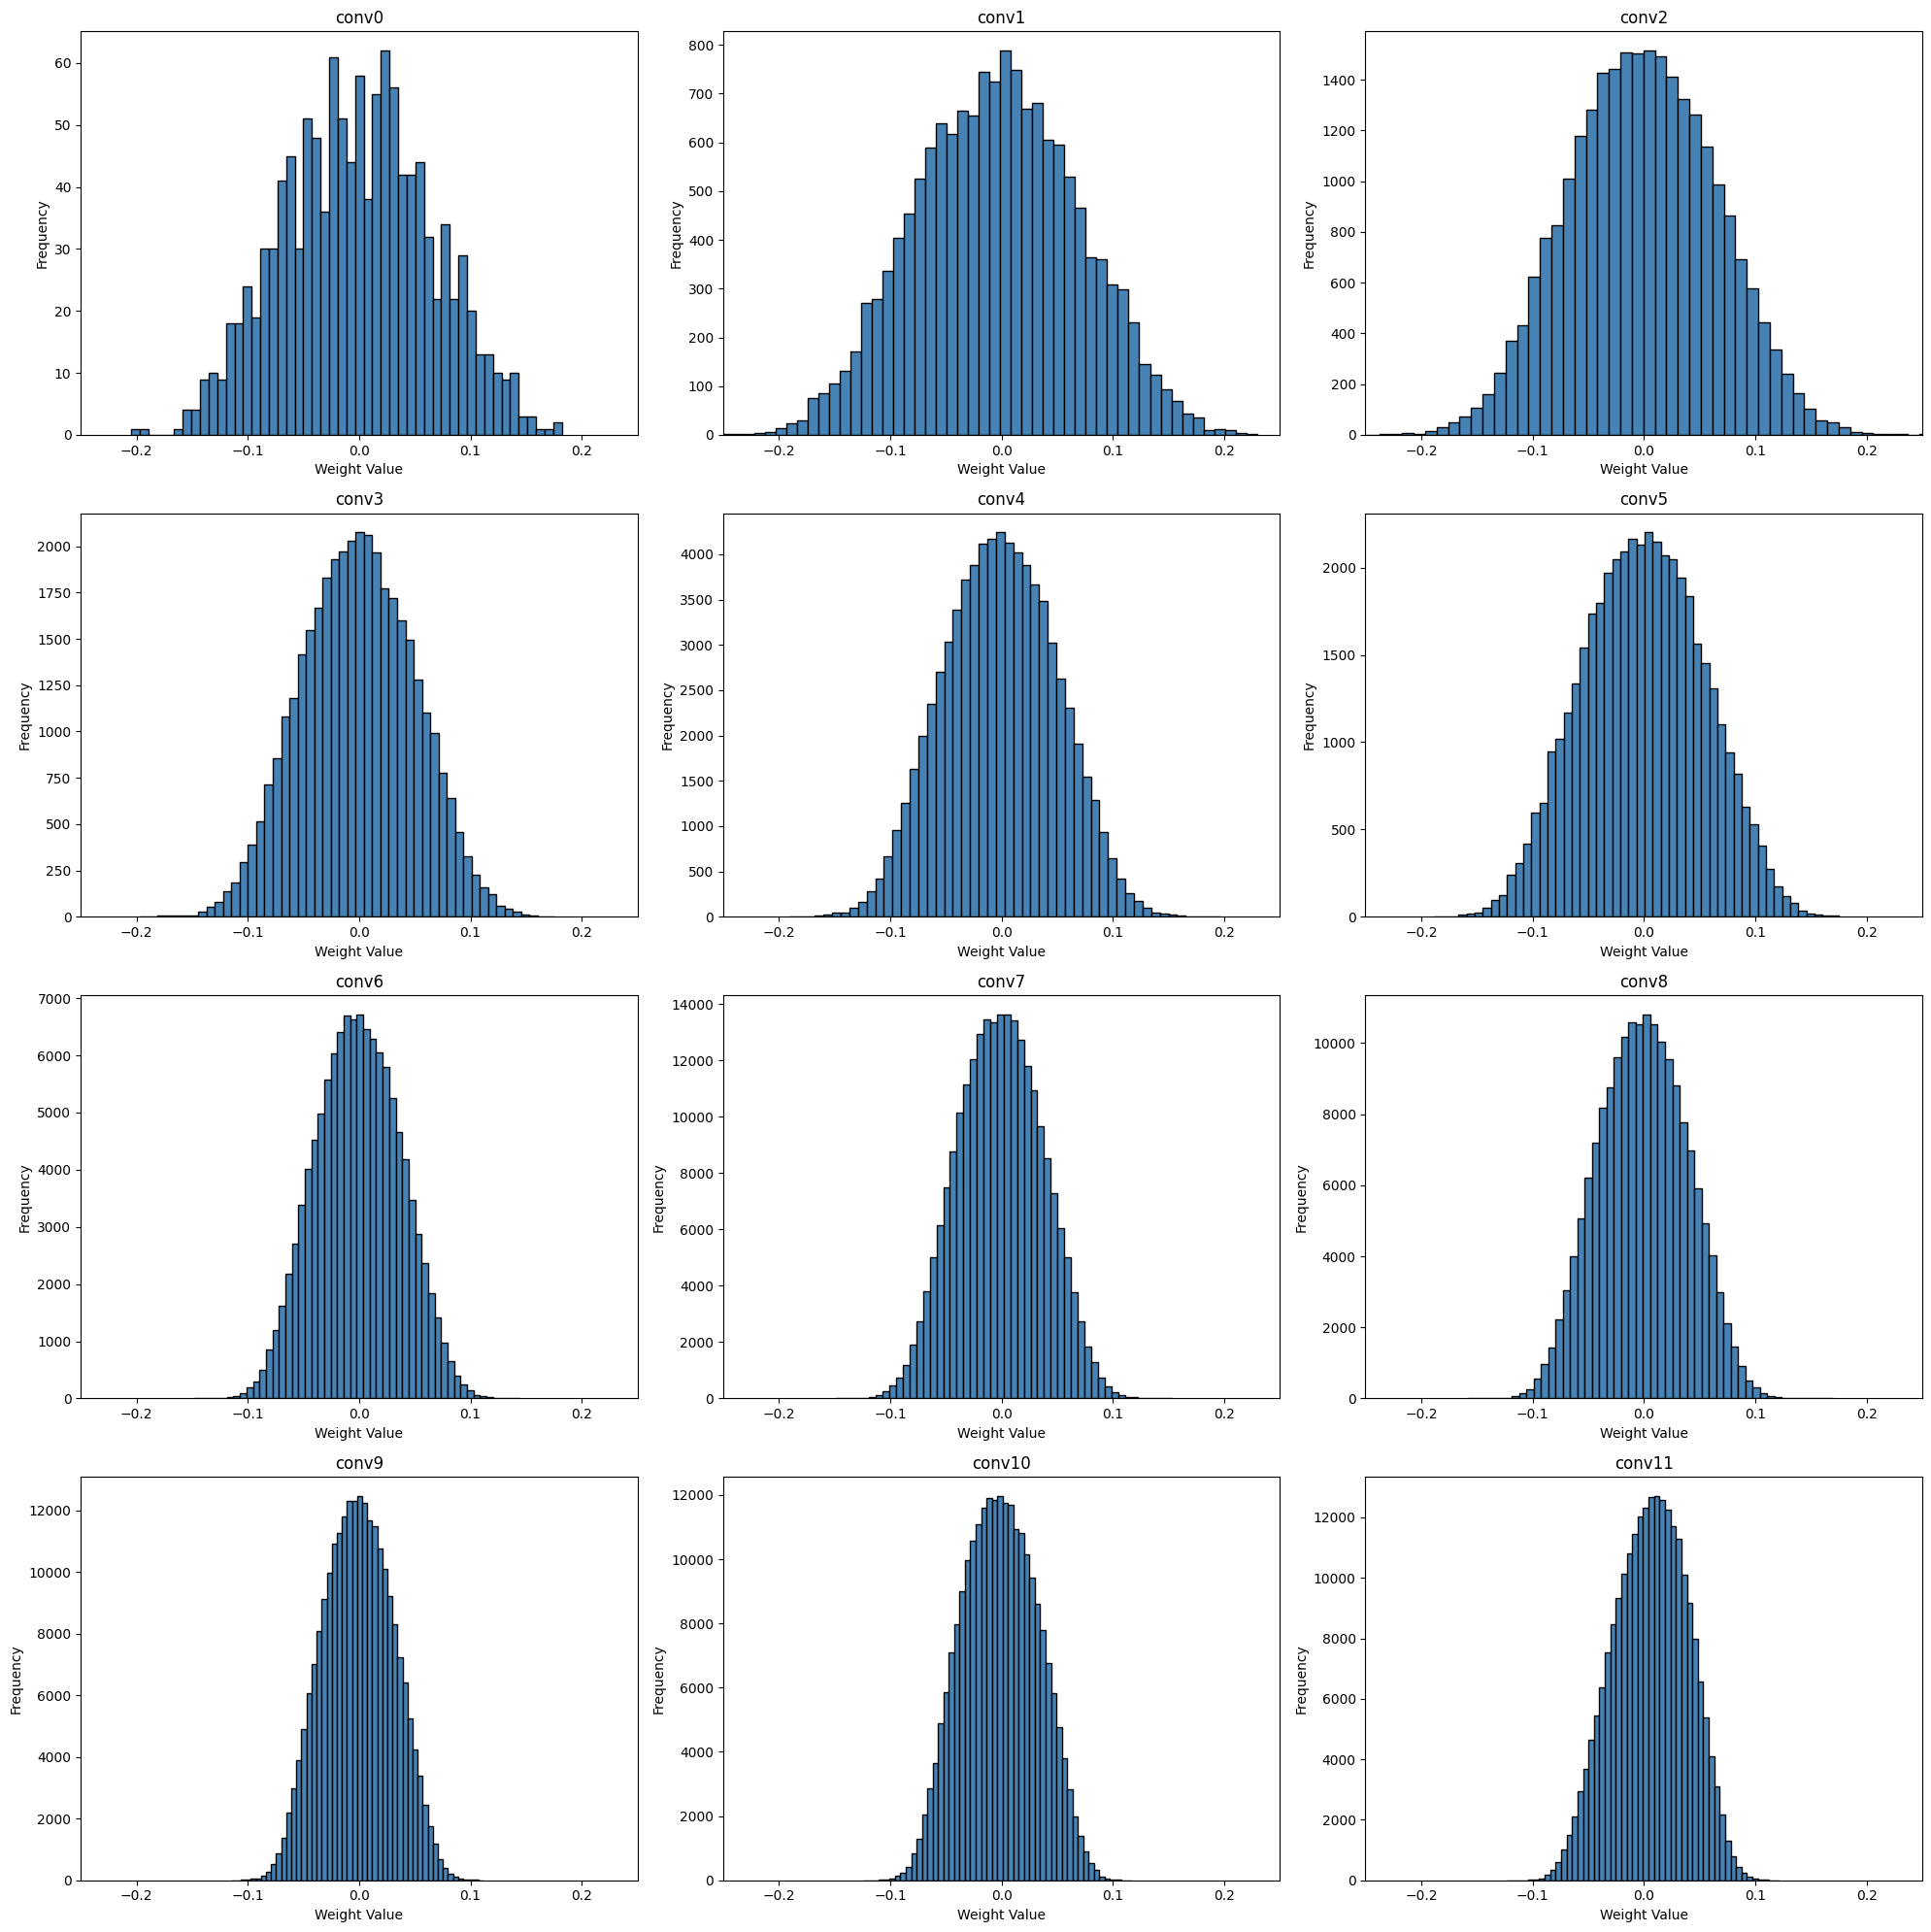
\includegraphics[width=1\linewidth]{report_images/kernel_dist_pp.png}
  \caption{\label{fig:kernel_dist_pp}Kernel Pruned Model Weights Distribution (Pre-Fine-tuning)}
\end{figure}
\FloatBarrier

\begin{figure}[h]
  \centering
  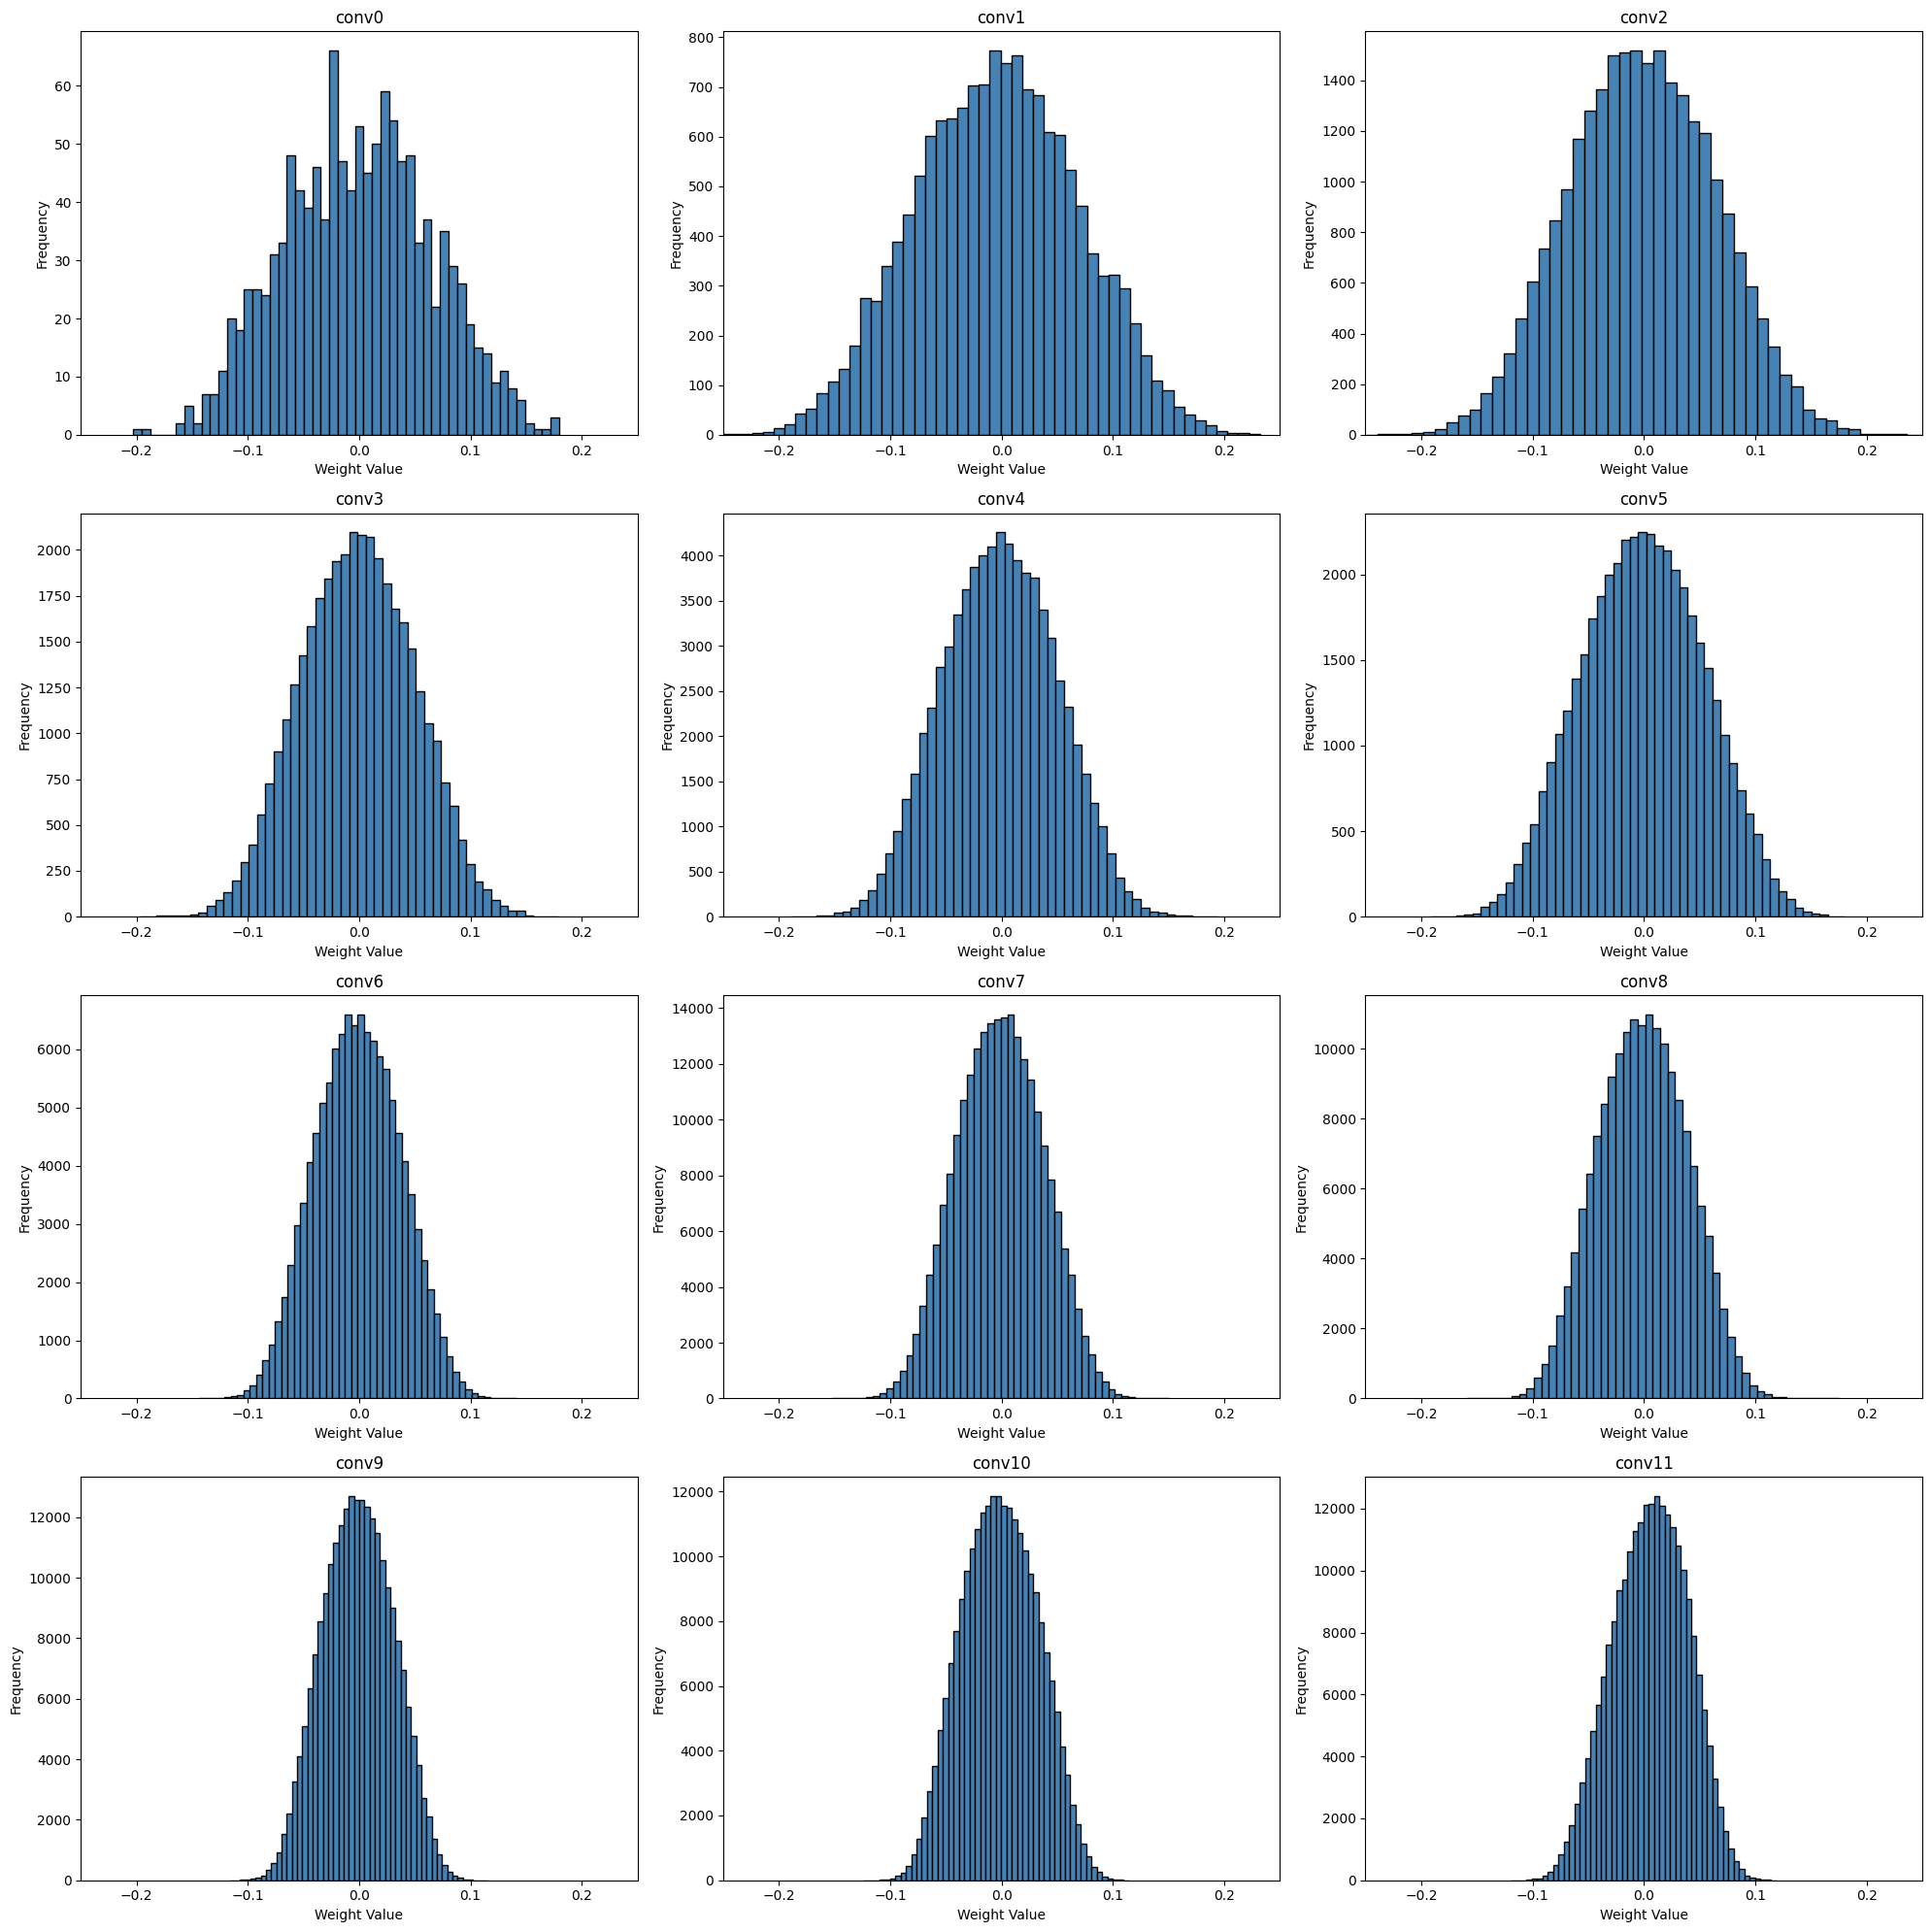
\includegraphics[width=1\linewidth]{report_images/kernel_dist_ft.png}
  \caption{\label{fig:kernel_dist_ft}Kernel Pruned Model Weights Distribution (Post-Fine-tuning)}
\end{figure}
\FloatBarrier

\begin{figure}[h]
  \centering
  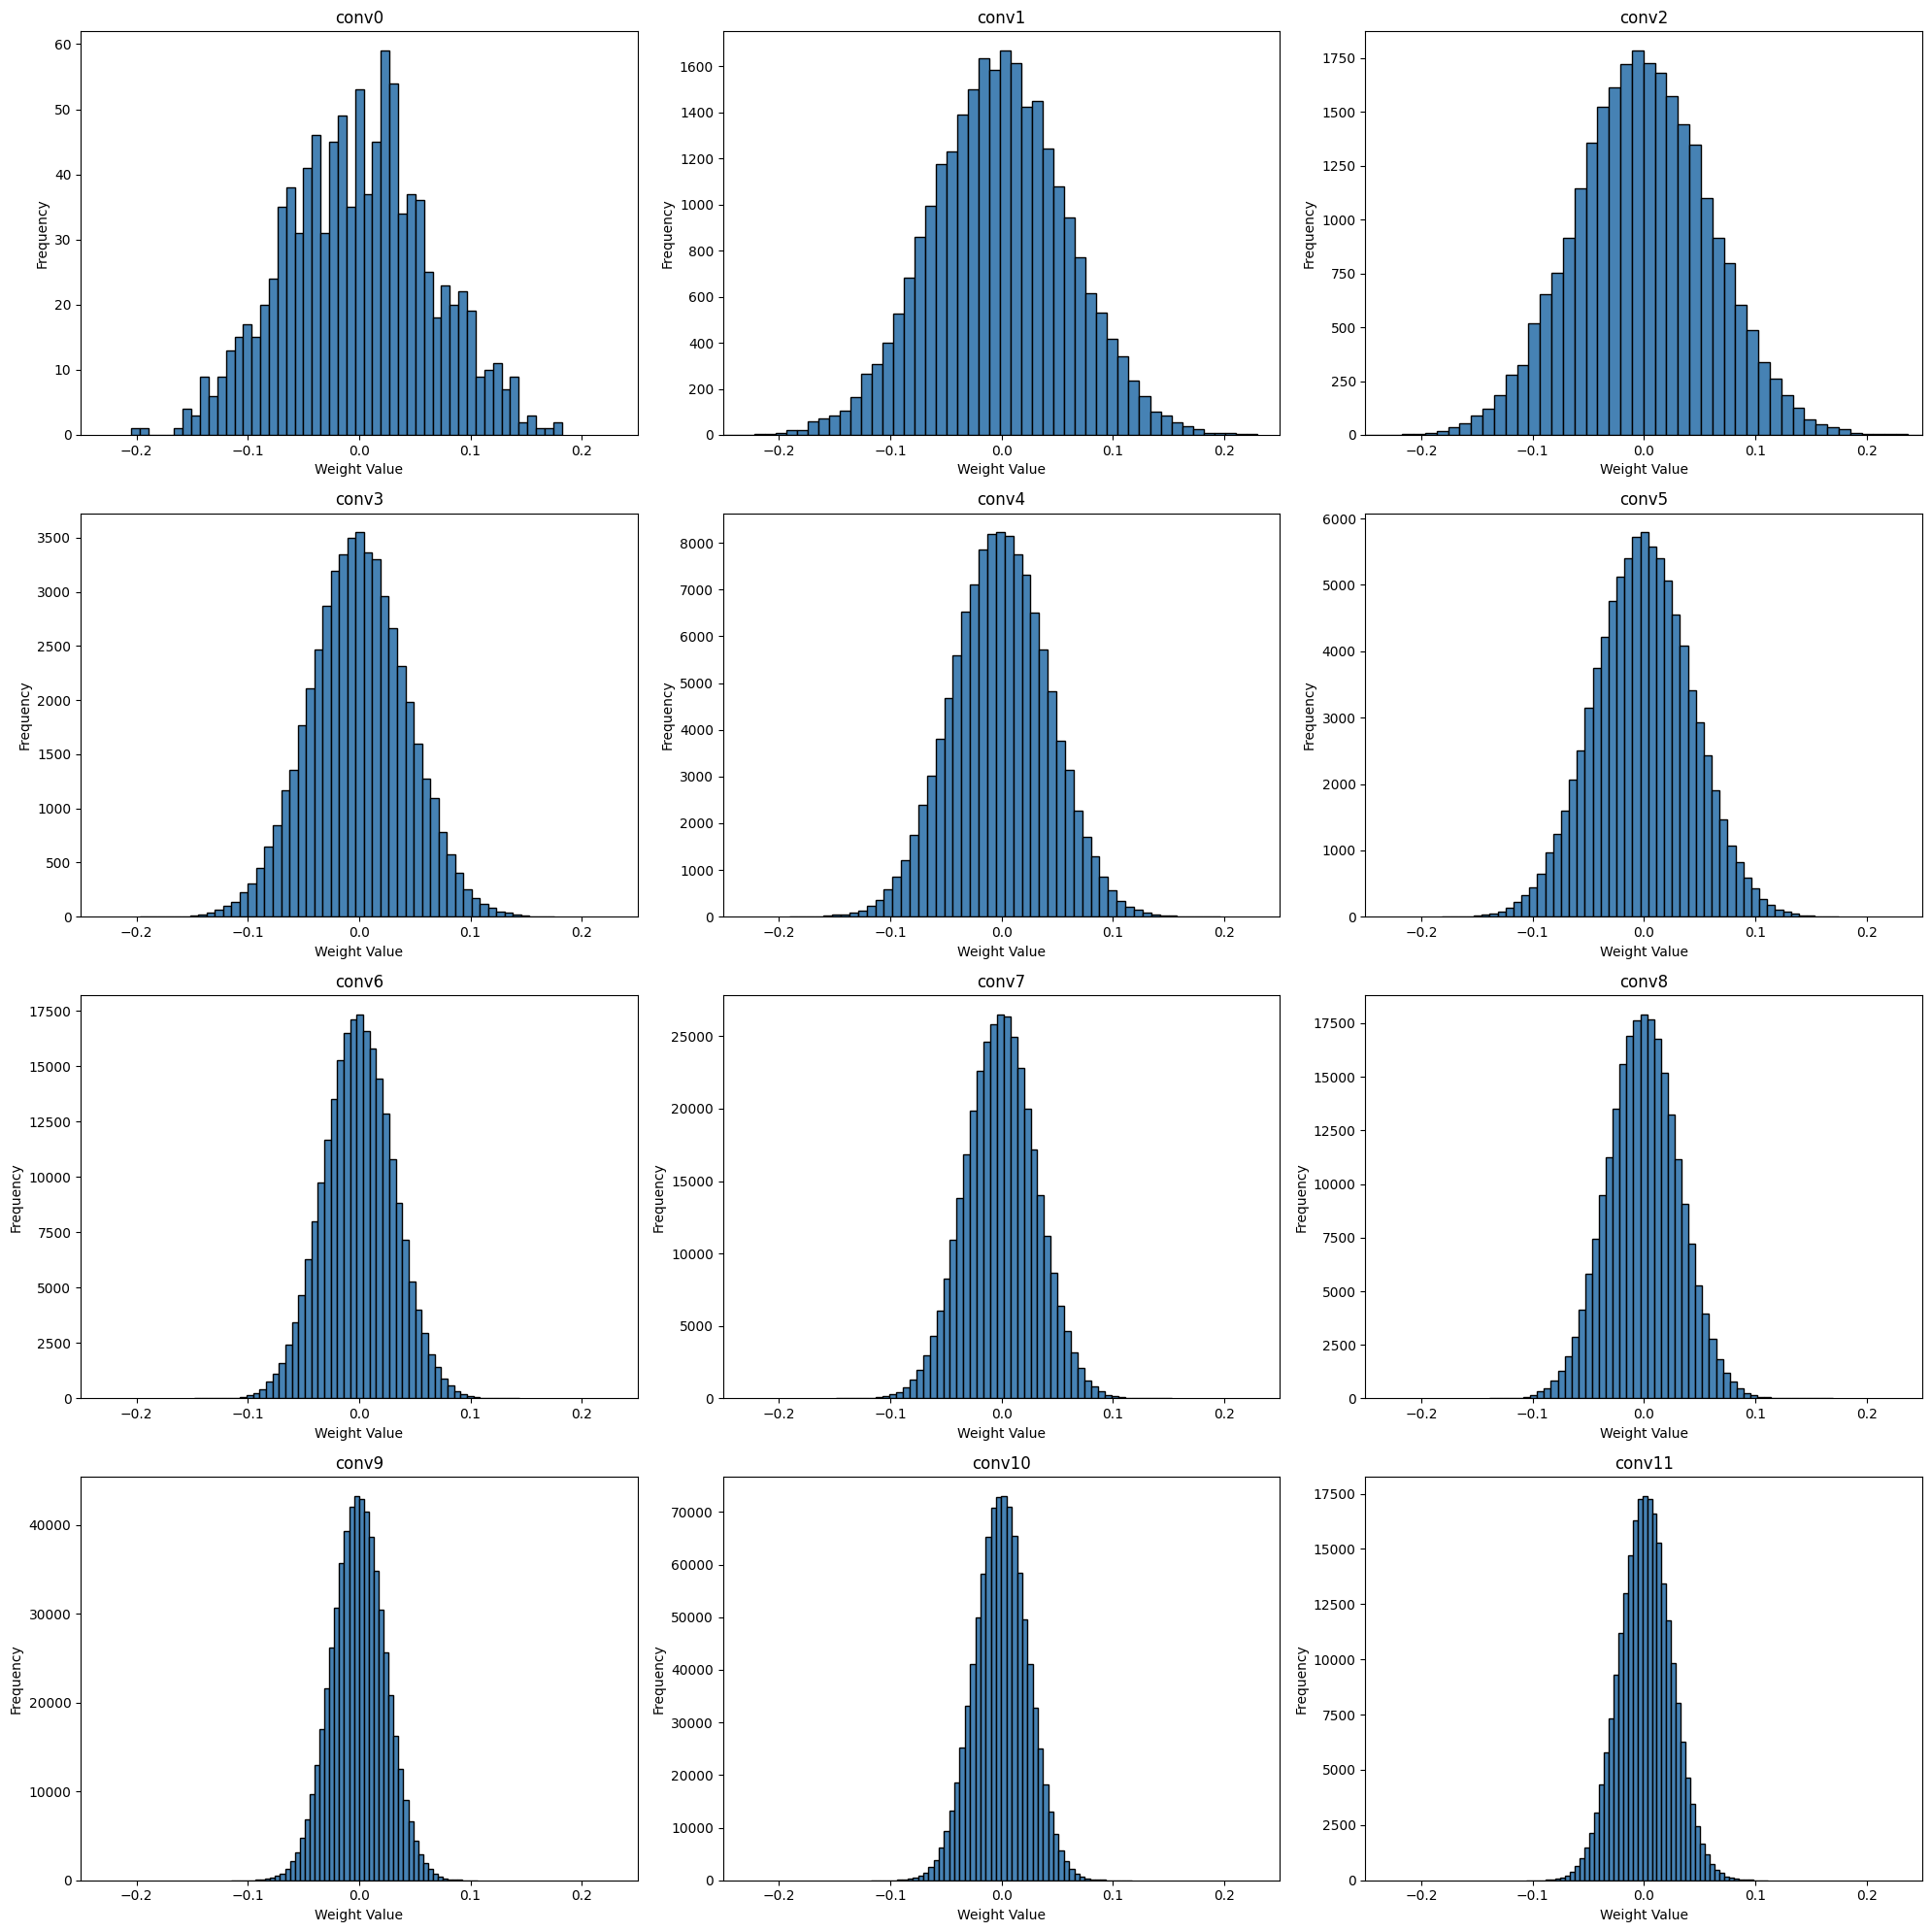
\includegraphics[width=1\linewidth]{report_images/filter_dist_pp.png}
  \caption{\label{fig:filter_dist_pp}Filter Pruned Model Weights Distribution (Pre-Fine-tuning)}
\end{figure}
\FloatBarrier

\begin{figure}[h]
  \centering
  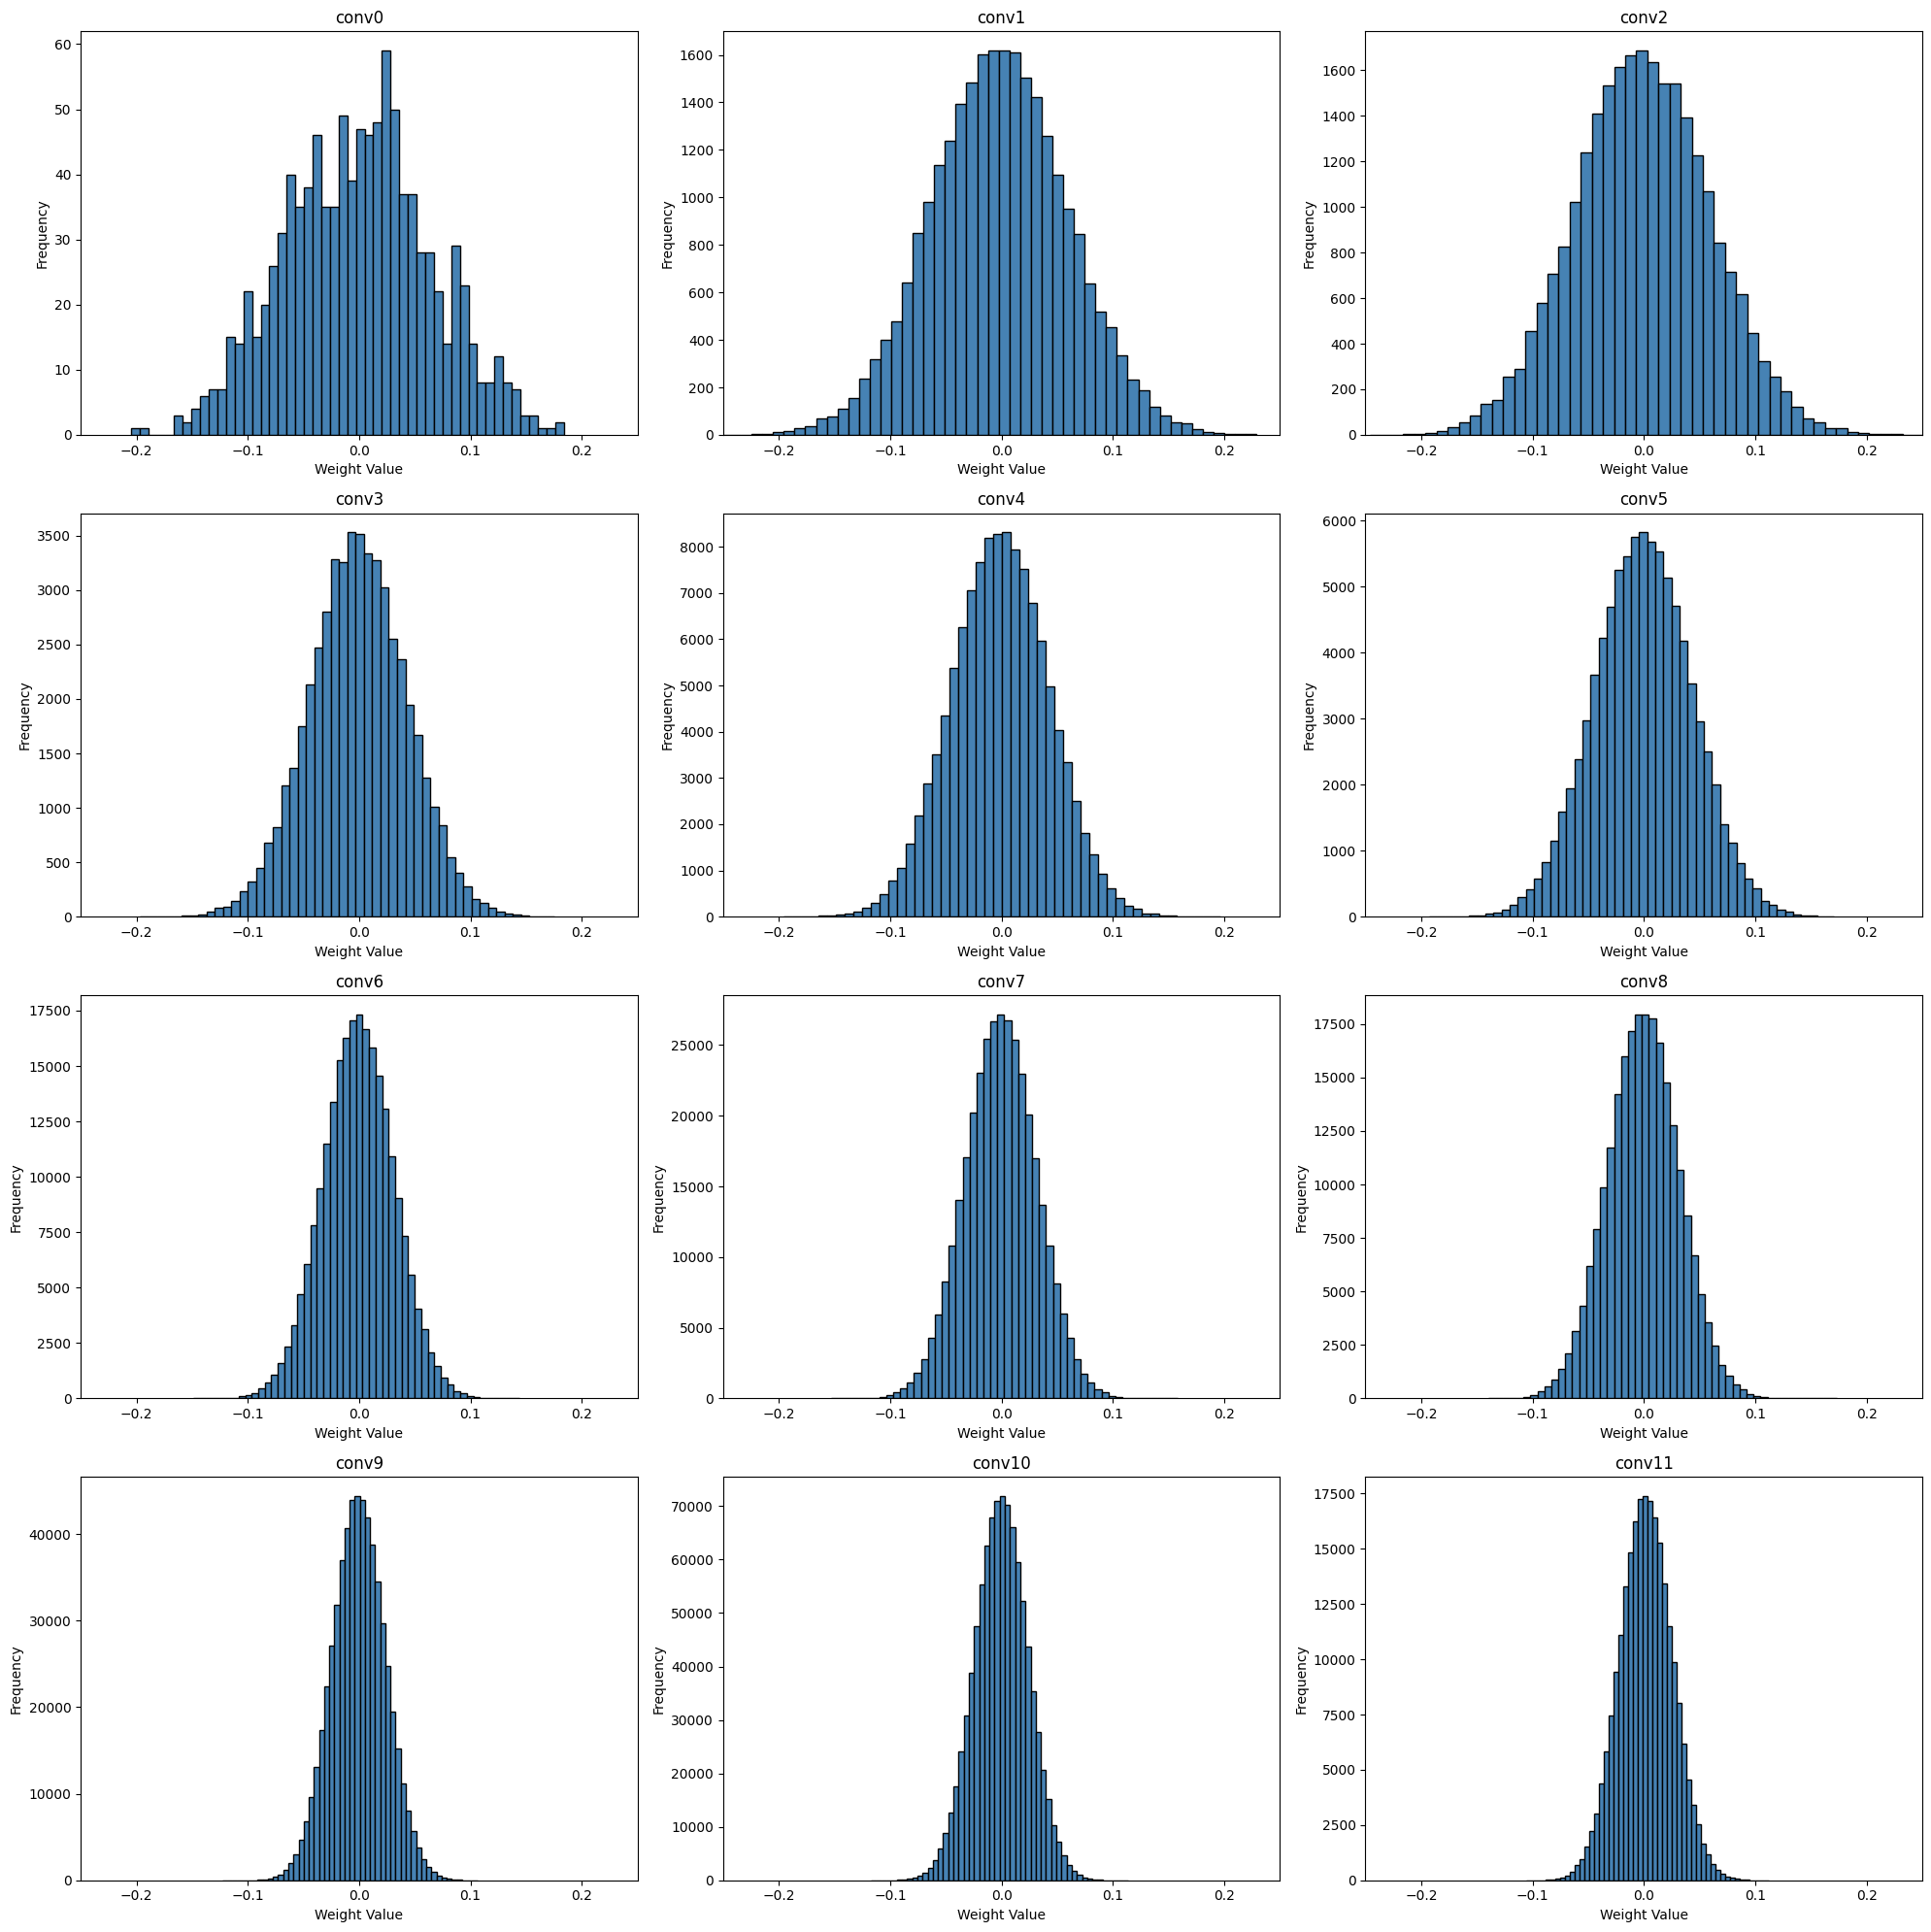
\includegraphics[width=1\linewidth]{report_images/filter_dist_ft.png}
  \caption{\label{fig:filter_dist_ft}Filter Pruned Model Weights Distribution (Post-Fine-tuning)}
\end{figure}
\FloatBarrier
\pagebreak

%%%%%%%%%%
\subsection{Activation Balances}
\label{activations}

\begin{figure}[h]
  \centering
  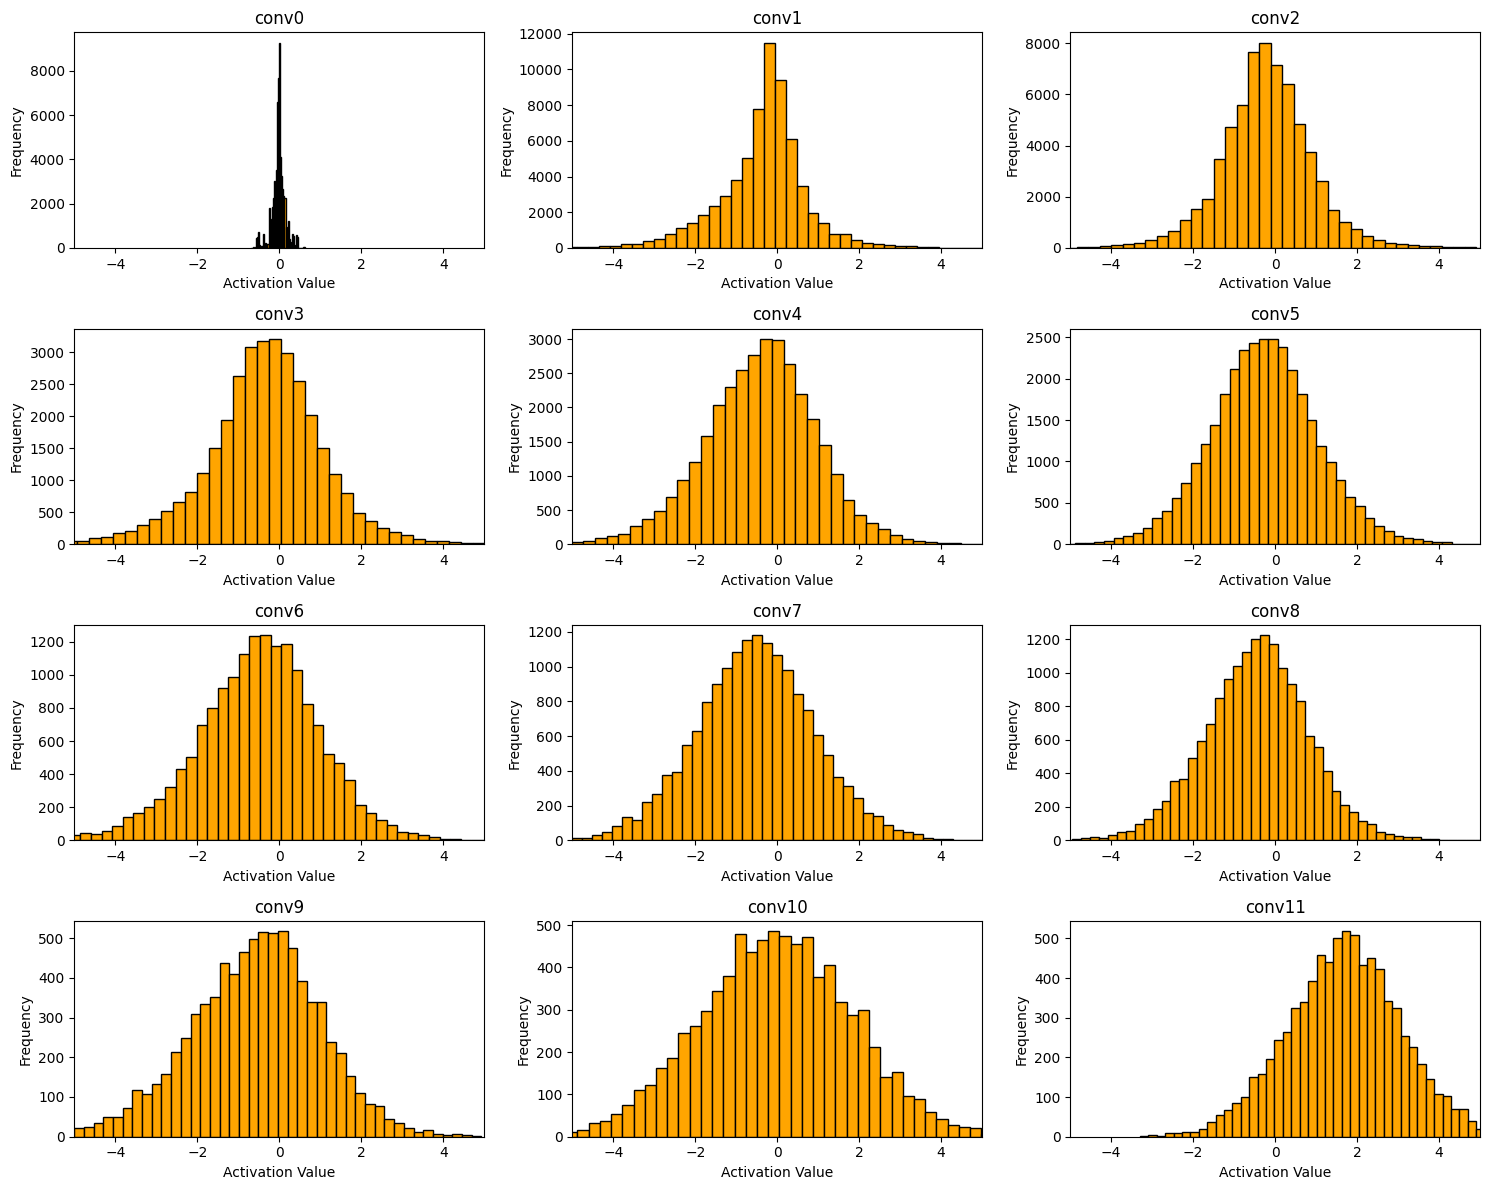
\includegraphics[width=1\linewidth]{report_images/unpruned_act.png}
  \caption{\label{fig:unpruned_act_dist}Un-pruned Model Activation Balance}
\end{figure}
\FloatBarrier

\begin{figure}[h]
  \centering
  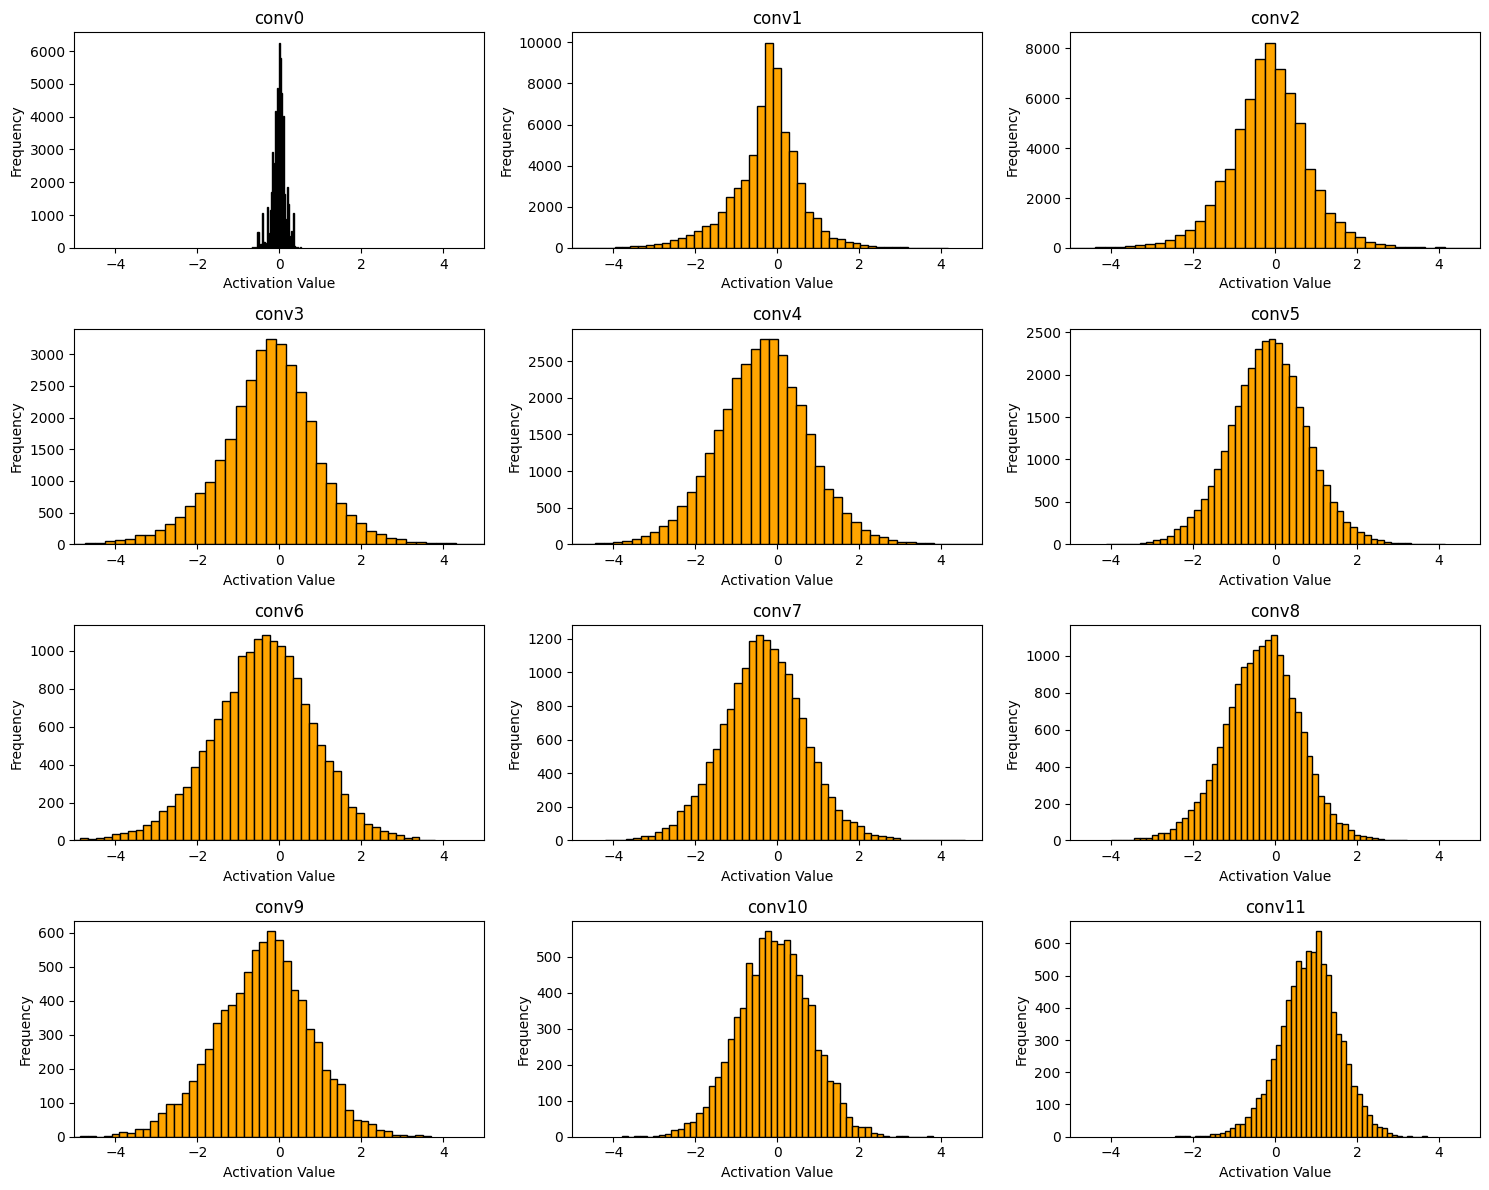
\includegraphics[width=1\linewidth]{report_images/fine_act_pp.png}
  \caption{\label{fig:fine_act_dist_pp}Fine-grained Model Activation Balance (Pre-Fine-tuning)}
\end{figure}
\FloatBarrier

\begin{figure}[h]
  \centering
  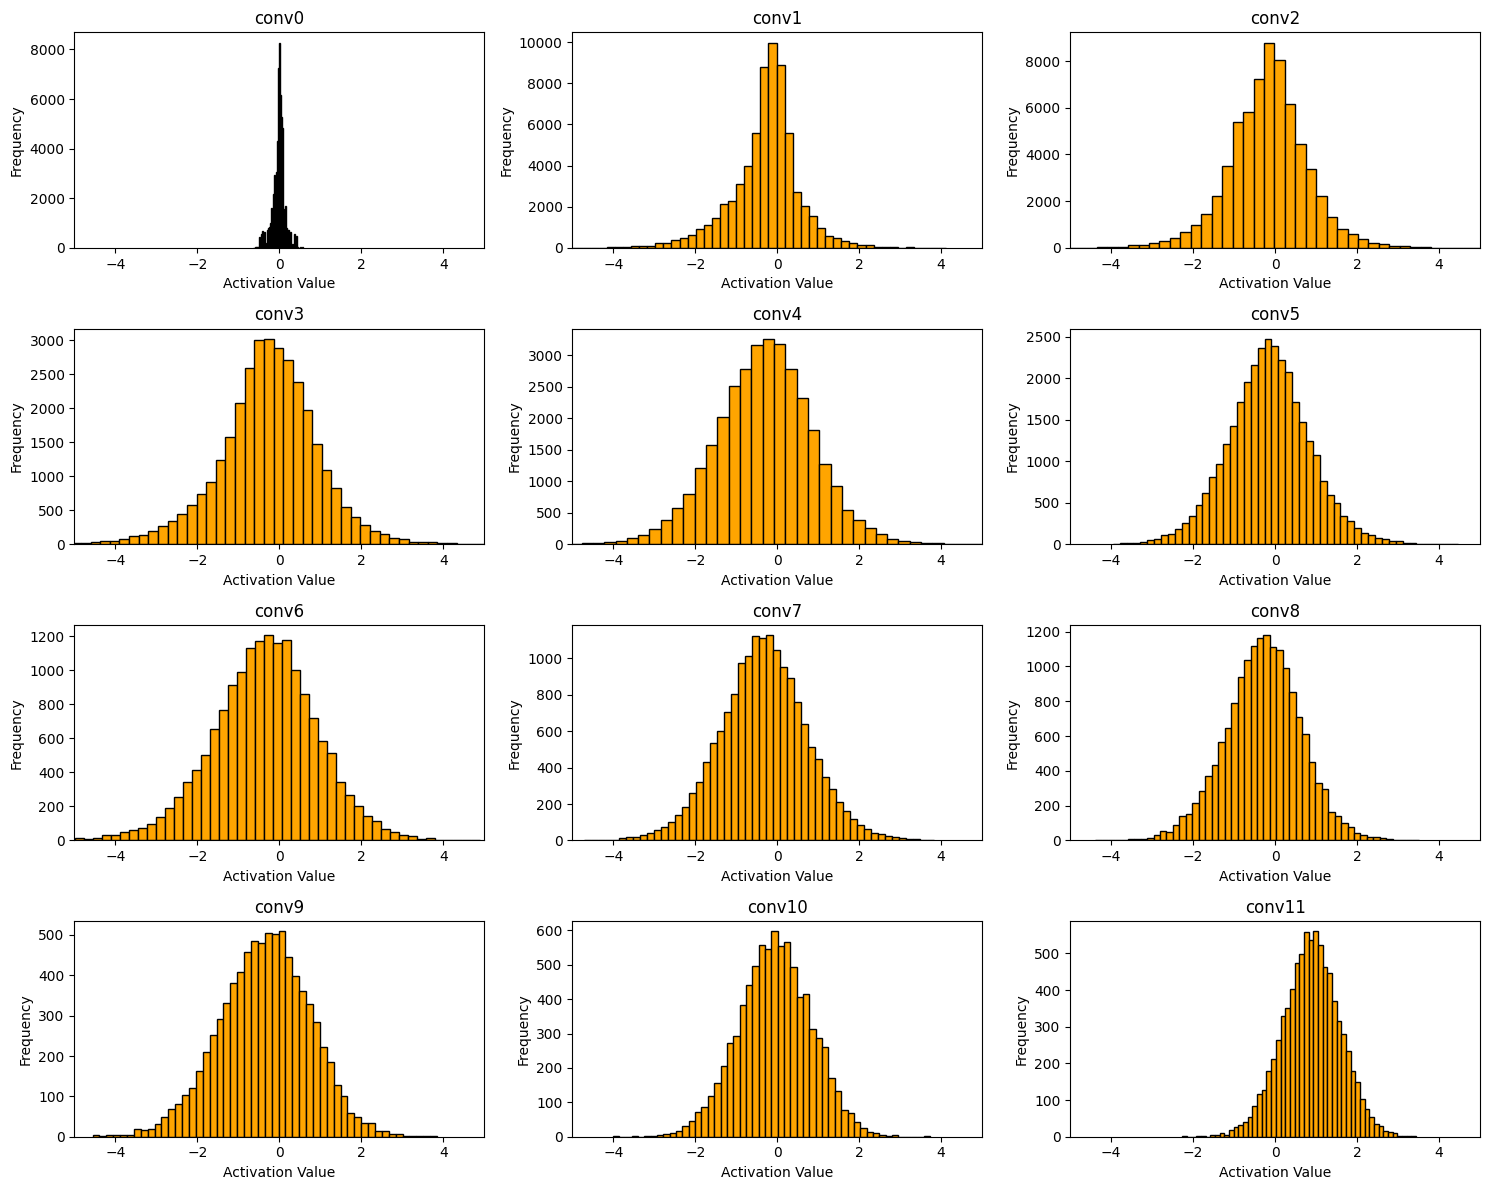
\includegraphics[width=1\linewidth]{report_images/fine_act_ft.png}
  \caption{\label{fig:fine_act_dist_ft}Fine-grained Pruned Model Activation Balance (Post-Fine-tuned)}
\end{figure}
\FloatBarrier

\begin{figure}[h]
  \centering
  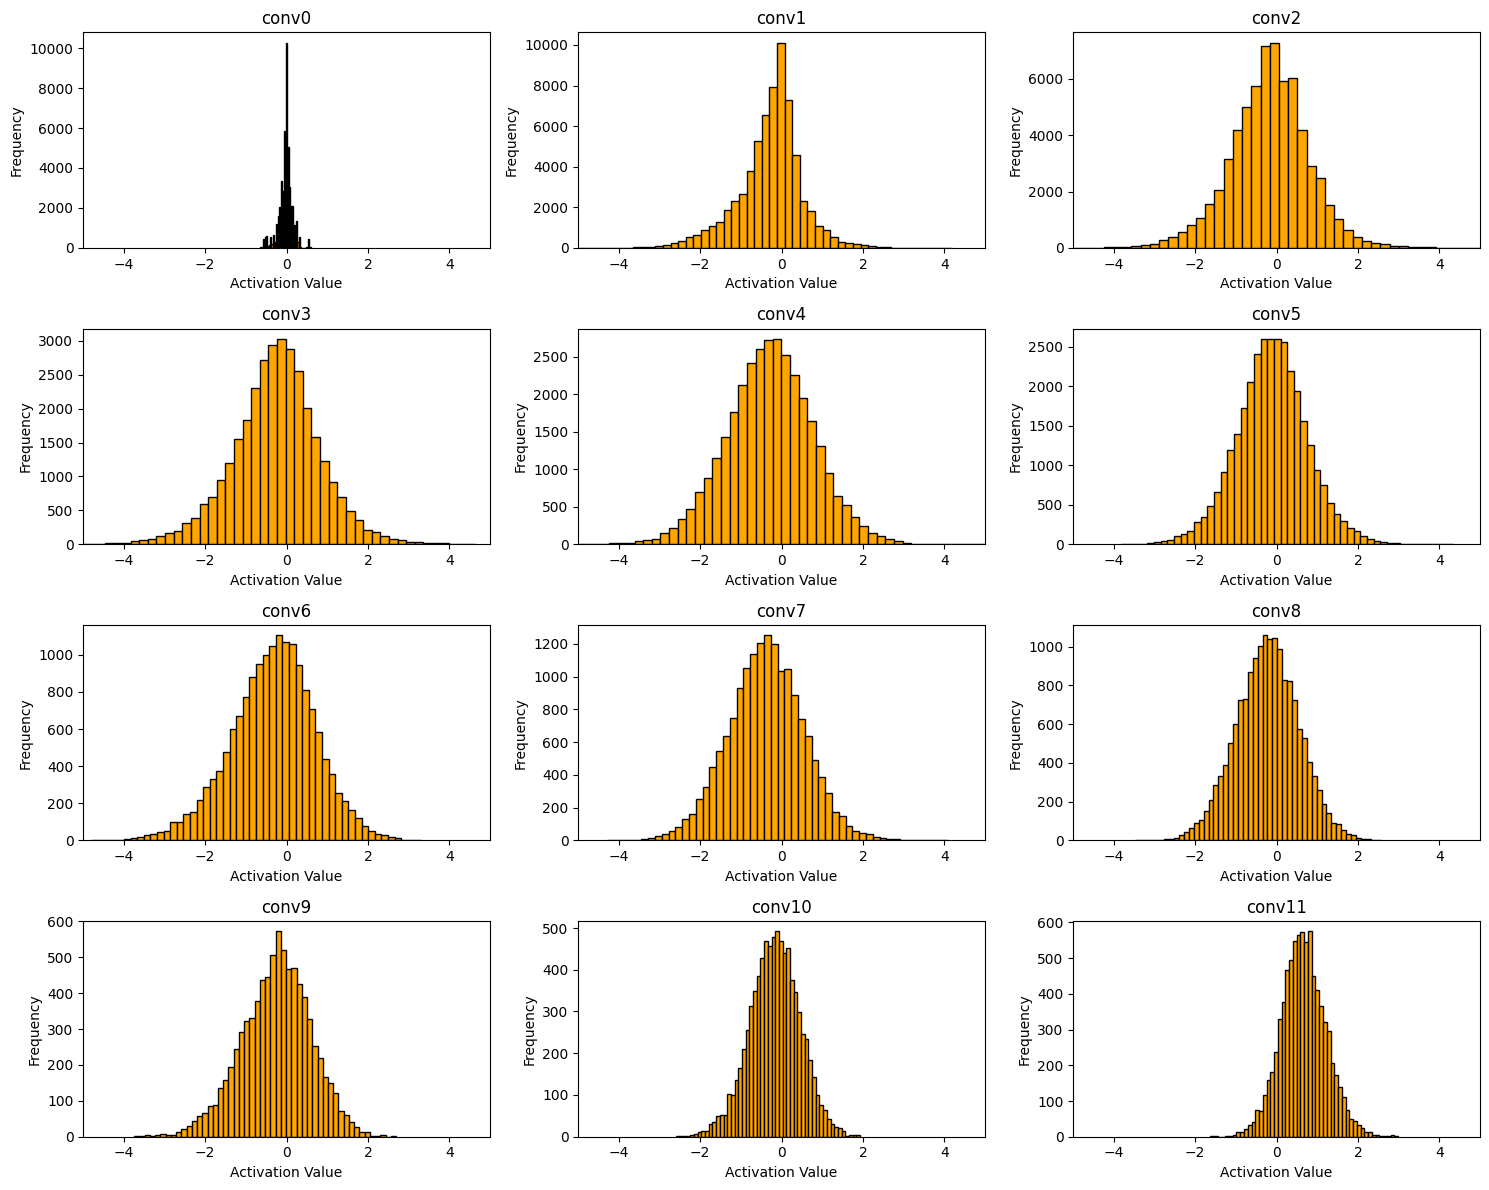
\includegraphics[width=1\linewidth]{report_images/kernel_act_pp.png}
  \caption{\label{fig:kernel_act_dist_pp}Kernel Pruned Model Activation Balance (Pre-Fine-tuning)}
\end{figure}
\FloatBarrier

\begin{figure}[h]
  \centering
  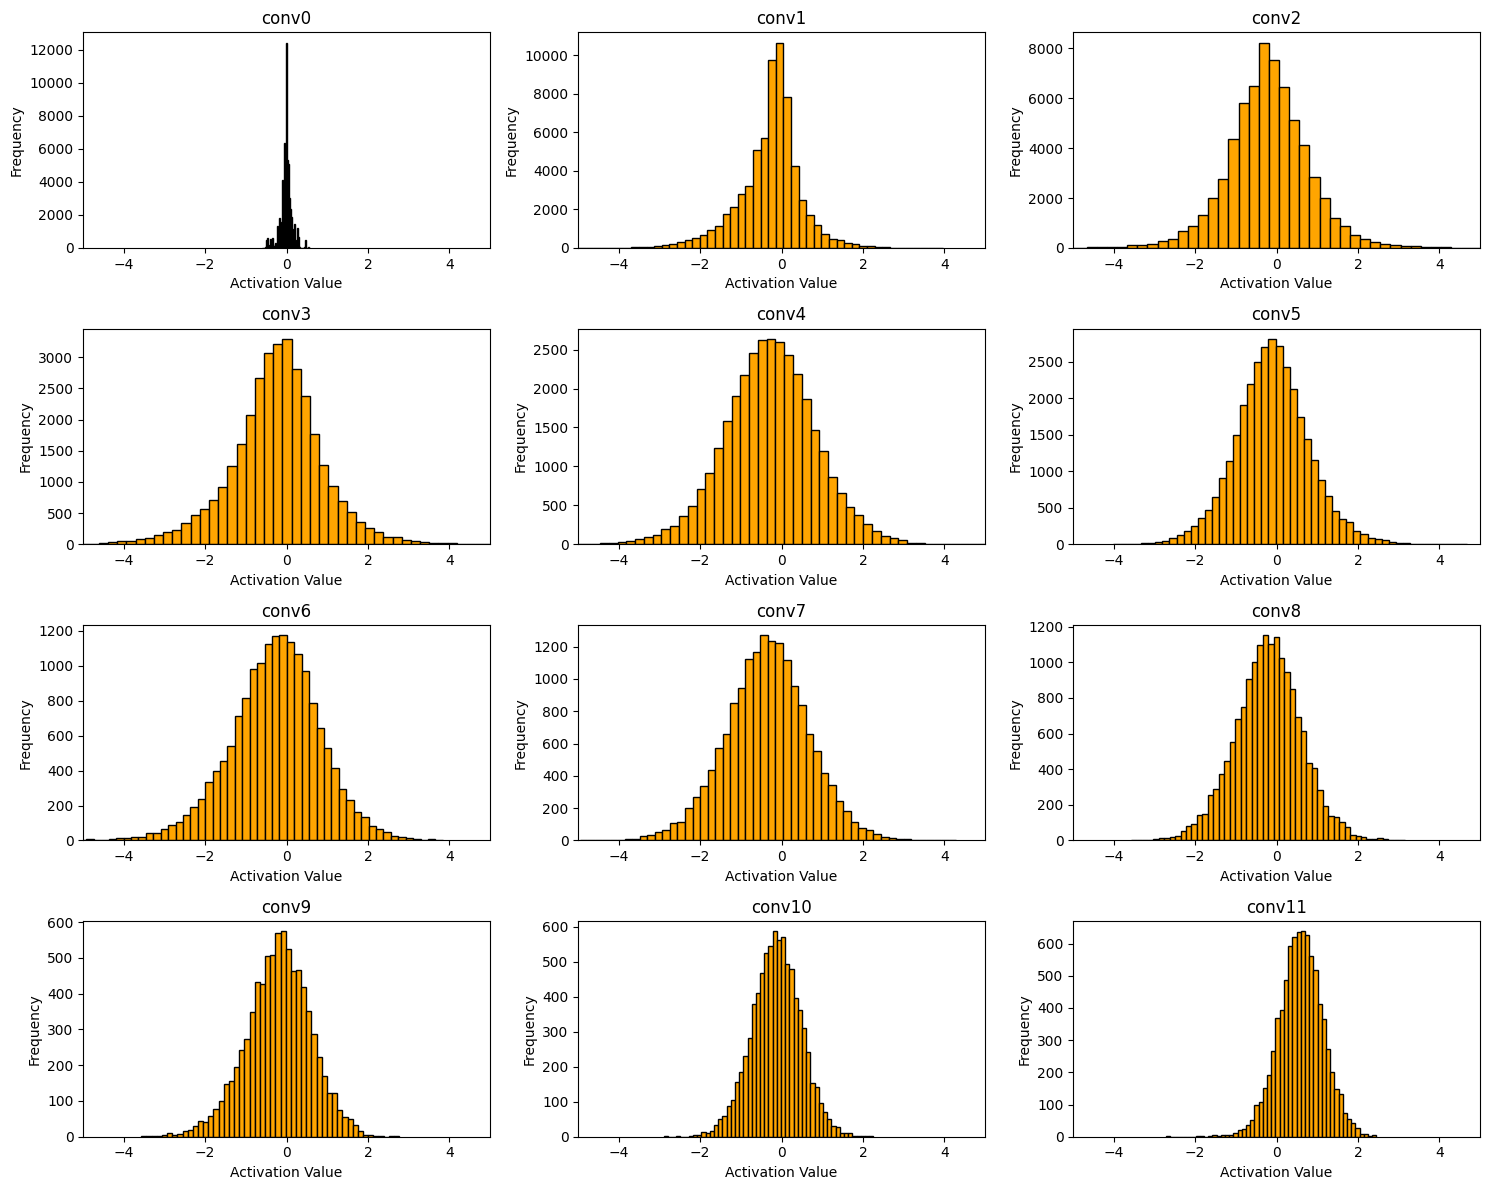
\includegraphics[width=1\linewidth]{report_images/kernel_act_ft.png}
  \caption{\label{fig:kernel_act_dist_ft}Kernel Pruned Model Activation Balance (Post-Fine-tuning)}
\end{figure}
\FloatBarrier

\begin{figure}[h]
  \centering
  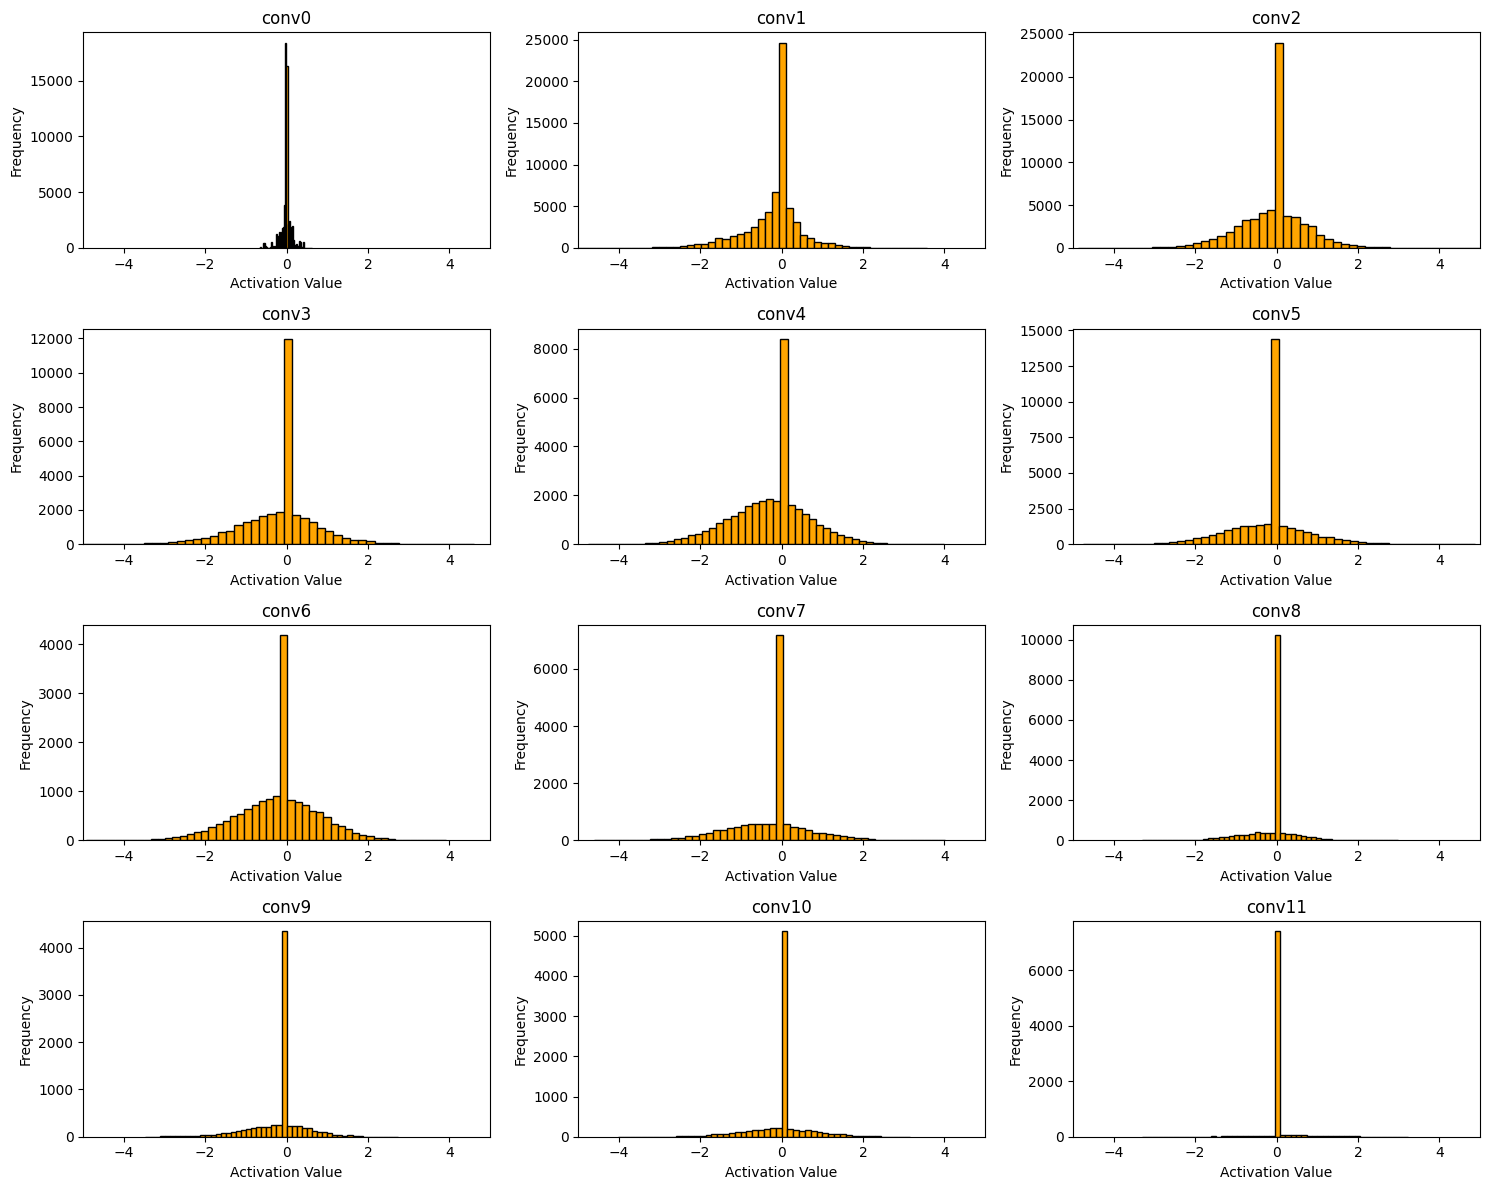
\includegraphics[width=1\linewidth]{report_images/filter_act_pp.png}
  \caption{\label{fig:filter_act_dist_pp}Filter Pruned Model Activation Balance (Pre-Fine-tuning)}
\end{figure}
\FloatBarrier

\begin{figure}[h]
  \centering
  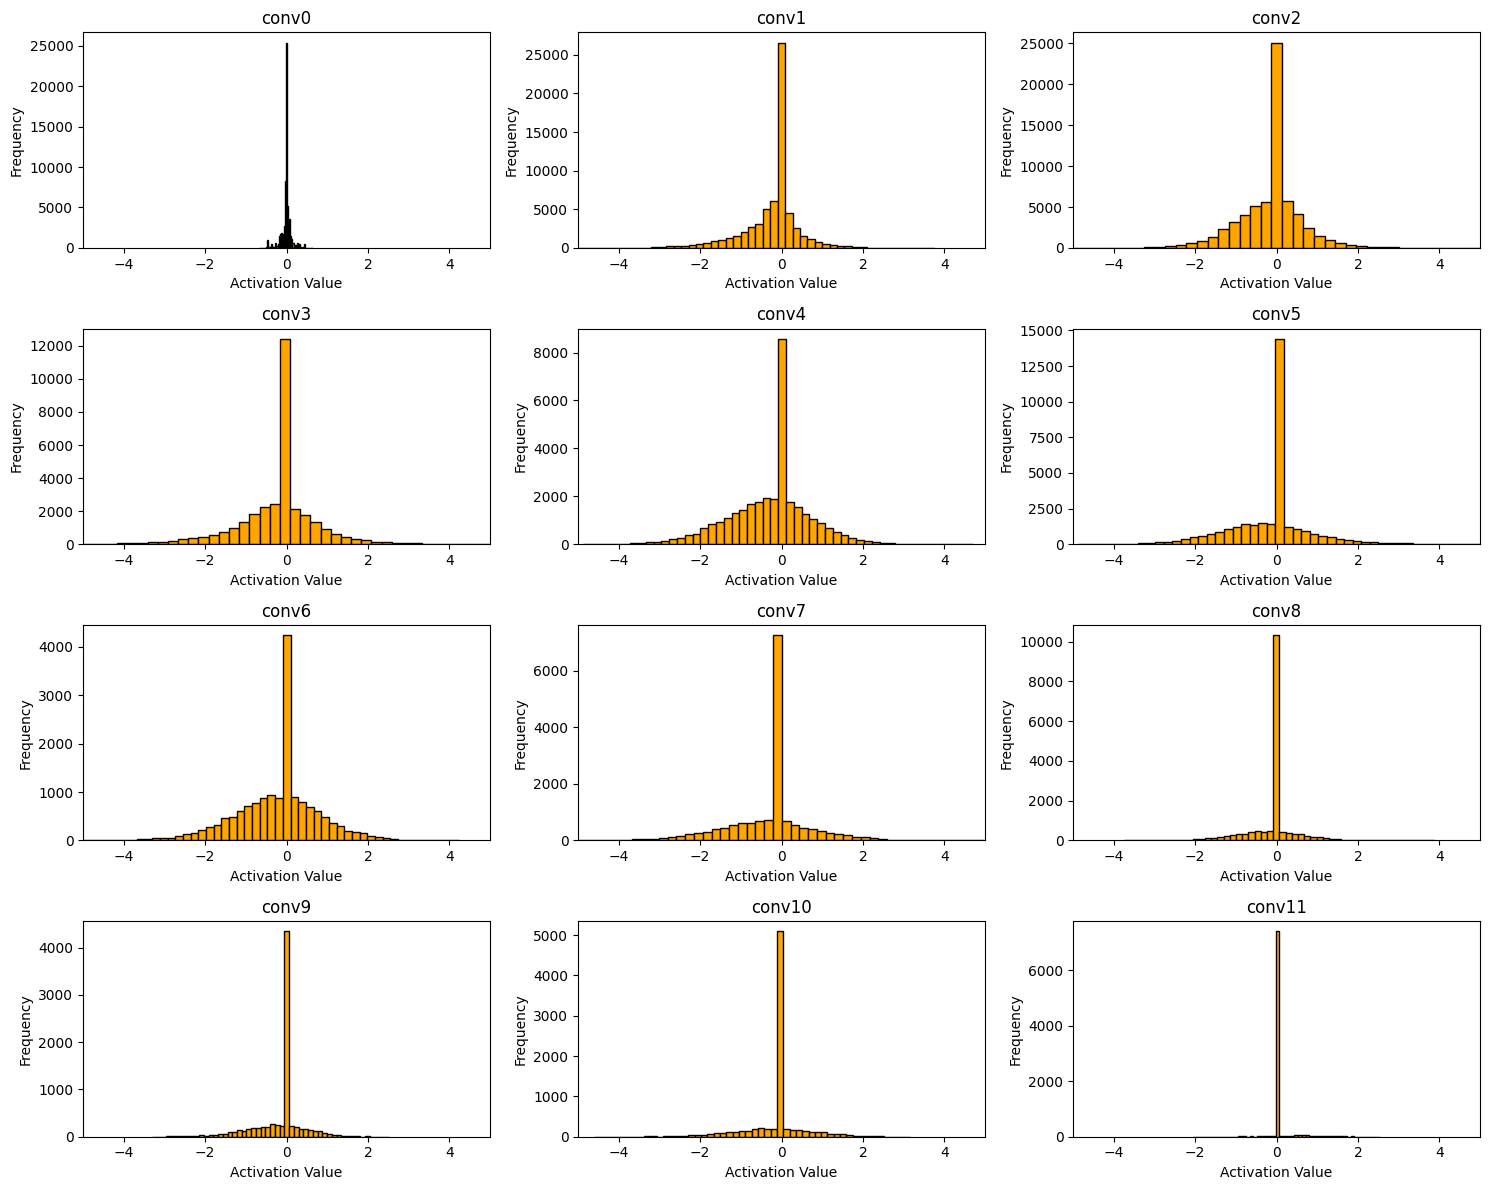
\includegraphics[width=1\linewidth]{report_images/filter_act_ft.png}
  \caption{\label{fig:filter_act_dist_ft}Filter Pruned Model Activation Balance (Post-Fine-tuning)}
\end{figure}
\FloatBarrier


\end{document}
